\documentclass[12pt, a4paper]{book}
\renewcommand{\baselinestretch}{1.5}

\usepackage{csvsimple}
\usepackage[french]{babel}
\usepackage{graphicx}
\usepackage[T1]{fontenc}
\usepackage{textcomp}
\usepackage{eurosym}
\usepackage{amsthm}

\newcommand{\Tc}{\mathcal{T}_c}
\newcommand{\Tv}{\mathcal{T}_v}
\newcommand{\E}{\mathcal{E}}
\newtheorem{prop}{Proposition}

\begin{document}




\tableofcontents

\newpage
\section{Introduction}
Le Plan d'Epargne Logement (PEL) est un produit financier relativement complexe qui permet d'acquérir des droits à des prêts pour financer un éventuel achat immobilier.  Il représente en fait une promesse de crédit à un taux prédéterminé. A ce titre, les droits à prêt dont bénéficient les épargnants sont des engagements qui doivent être comptabilisés depuis l'entrée en vigueur des nouvelles normes comptables internationales IAS-IFRS depuis l'année 2005.

Lorsque un établissement de crédit offre des plans d'épargne logement, il est exposé à deux type de risques :

Le premier est lié à l'obligation de rémunérer l'épargne dans le futur à un taux fixé à l'ouverture du contrat.

Le deuxième, lié à l'octroi d'un crédit à un taux déterminé fixé aussi à l'ouverture du contrat.

L'évaluation des engagements des établissements dépendant des comportements futurs des souscripteurs, les établissements utilisent les modalités de calcul qu’ils jugent les plus appropriées mais ils doivent prendre en compte le comportement des souscripteurs épargnants, le comportement des souscripteurs exerçant leurs droits à prêts et la courbe des taux observables sur le marché et ses évolutions anticipées.
 
La constitution de la provision est donc un processus qui comporte deux étapes principales. La première est la modélisation du comportement des épargnants face à différentes conditions de l'économie et la seconde est la modélisation de l'évolution des taux du marché.

Dans le document présent, nous décrivons une méthode pour calculer la provision. Dans la première partie, nous étudions le problème de la modélisation du comportement des épargnants. Nous allons nous concentrer sur l'effet qui pourrait être produit si on ne prend pas en compte des variables propres de chaque plan d'épargne logement. Au regard de la volumétrie importante des contrats dont une institution financière peut disposer, la considération de l'historique des encours au niveau unitaire devient très compliquée. Il est normal d'agréger les encours par strate, c'est à dire, par génération mensuelle d'ouverture. Ce choix est raisonnable pour simplifier les calculs mais élimine les effets qui ne sont mesurables qu'au niveau unitaire. 

Dans la deuxième partie, nous allons modéliser les taux du marché, ce qui, avec la modélisation comportementale faite dans le premier chapitre, nous permettra de construire la provision en fonction de l'incertitude liée aux conditions du marché. Ceci, dans le respect des conditions imposées par le Conseil National de la comptabilité dans son avis N° 2006-02 du 31 mars 2006 relatif à la comptabilisation des plans d'épargne-logement \cite{CNC1}.

En raison de l'utilisation de taux d'intérêt de maturités différentes, nous allons utiliser un modèle de taux composé de plusieurs facteurs (voir le chapitre 4 de Brigo et Mercurio \cite{BM}). Nous élaborerons les outils nécessaires pour utiliser les données historiques sur les taux d'intérêt afin de calibrer les paramètres du modèle, contrairement à la méthode présentée dans \cite{BM} où le modèle est calibré en utilisant la valeur présente de quelques instruments financiers, selon une optique de probabilité risque neutre.

Le calcul de la provision sera effectué dans trois contextes différents qui nous permettront d'estimer les effets d'une absence de prise en compte des variables explicatives dans la modélisation comportementale réalisée au chapitre \ref{chap1}.

Tout au long de ce document, nous allons travailler uniquement sur la provision liée à la phase d'épargne du Plan d'épargne logement. La provision liée à la partie crédit est mois importante dans le contexte de taux d'intérêt bas qui se présente actuellement. En effet, nous vivons actuellement dans une période où les taux du marché sont inférieurs aux taux d'emprunt imposés par les plans d'épargne logement, les droits à prêt sont négligeables car la plupart des détenteurs de PEL préfèrent emprunter sur le marché plutôt que de les utiliser.

\chapter{Modélisation comportementale}
\label{chap1}
\section{Introduction}

Le but de ce chapitre est de détecter et mesurer des éléments du comportement des propriétaires des plans d'épargne logement afin de modéliser et d'estimer les encours futurs, c'est à dire, le montant d'argent épargné dans le mois à venir. 

La modélisation des encours futurs est l'étape la plus importante pour la construction de la provision, elle permet de calculer le résultat futur de l'établissement financier proposant les plans d'épargne logement, en fonction de différents paramètres économiques, tels que, par exemple, l'évolution des taux du marché. 

Chaque mois, les encours seront calculés à l'aide de deux séries mensuelles, le taux de clôture et le taux des versements. La première mesure la proportion des encours supprimés dans un mois donné et le second mesure la proportion des montants qui sont ajoutés. Les deux taux sont calculés par "strate" de plans d'épargne logement, qui est défini comme l'ensemble des plans qui partagent le même mois d'origine.
Par exemple, la "strate" de mai 2005 fait référence à tous les plans d'épargne logement qui ont été ouverts ce mois-là. 

Les taux de clôture et des versements sont estimés à partir des observations mensuelles d'une période de vingt ans. Le Conseil National de la Comptabilité, CNC, dans son avis N° 2006-02 du 31 mars 2006 relatif à la comptabilisation des plans d'épargne-logement \cite{CNC1}, établit que les paramètres d'estimation des comportements futurs d'épargne et de crédit doivent résulter d'observations historiques de longue période. Les établissements utilisent les modalités de calcul qu'ils jugent les plus appropriées dans la mesure où elles respectent les conditions décrites ci-après.
Elles doivent prendre en compte le comportement des souscripteurs épargnants, le comportement des souscripteurs exerçant leurs droits à prêts, une estimation du montant et de la durée des emprunts qui seront mis en place dans le futur, la courbe des taux observables sur le marché et ses évolutions raisonnablement anticipées et elles doivent présenter une certaine stabilité dans le temps.

Nous allons nous concentrer sur la phase d'épargne, pour cela, nous allons supposer que les épargnants ne convertissent pas leur compte d'épargne en crédit. Cette hypothèse est tout à fait vraie dans le contexte des taux d'intérêt actuellement observés, en effet, nous vivons actuellement dans une période où les taux du marché sont inférieurs aux taux d'emprunt imposés par les plans d'épargne logement, cela décourage les gens d'utiliser la possibilité de convertir leur épargne en crédit. La provision pour la phase de crédit était pertinente dans le passé, lorsque les taux d'intérêt étaient élevés. Pour plus de détails, je suggère l'article écrit par Baud et al. \cite{BetAl}.

En plus d'éliminer la provision pour la phase de crédit, nous ferons d'autres simplifications. Afin de se concentrer uniquement sur la modélisation comportementale, nous allons supposer que les plans d'épargne logement ne sont pas soumis à la fiscalisation et qu'ils n'ont pas des primes d'État. Cette dernière hypothèse est vraie pour les dernières générations. 

La modélisation comportementale se concentrera sur l'effet de la non prise en compte des variables propres de chaque PEL. Au regard de la volumétrie importante des PEL dont une institution financière peut disposer, la considération de l'historique des encours au niveau unitaire devient très compliquée. Il est normal d'agréger les encours de PEL, par strate, c'est à dire, par génération mensuelle d'ouverture. Ce choix est raisonnable pour simplifier les calculs mais élimine les effets qui ne sont mesurables qu'au niveau unitaire. 

Dans la première partie, nous allons détailler la base de données utilisée pour l'estimation des taux de clôture et de versements. La base de données est fictive, ne contient pas de données réelles, elle a été générée à partir de simulations de plans d'épargne logement individuels. Chaque PEL a été généré sur la base d'un projet d'achat immobilier qui prend en compte une quantité à épargner dans un temps souhaité pour chaque client à la date d'ouverture du PEL. Ces variables ne sont plus observables lors de l'agrégation par strates mensuelles. Les clients font des versements ou décident de clôturer le PEL, par rapport à leur projet et aux conditions observées de taux de marché.

Dans la deuxième partie nous allons modéliser les taux de clôture et des versements à l'aide d'une régression non paramétrique par noyau. Ce modèle a été choisi parce qu'il est facile à mettre en œuvre et qu'il s'est avéré efficace lorsqu'il y a un nombre important d'observations. Le choix des paramètres (la fenêtre de lissage) est donné dans un contexte de "machine learning", séparant les données dans une base d'apprentissage où le modèle est implémenté et ensuite testé dans l'autre partie nommée base de test (il s'agit du "train data" et du "test data"). 

Dans une troisième partie, nous ferons une analyse des résidus de la régression non paramétrique. Cette étude va nous permettre de simuler les taux de clôture et des versements de manière plus correcte. Les simulations seront utilisées pour le calcul de la provision dans le chapitre \ref{chap2}.

Dans cette section, nous étudierons l'effet de la négligence des caractéristiques individuelles des contrats des plans d'épargne logement, à savoir, les variables {\it Montant souhaité} et {\it Durée Souhaité}, sur la considération d'encours agrégés par génération mensuelle de production.  

Finalement, afin d'isoler l'effet d'une utilisation de la régression non paramétrique, qui produit elle-même une erreur d'estimation, nous allons reconstruire la base de données mais avec une population homogène, où tous les épargnants ont le même projet immobilier et donc, l'effet des variables propres à chaque PEL est moins importante. Nous comparerons la performance de la régression non paramétrique dans les deux bases de données construites. 

\section{Simulation des clôtures et versements}

Dans cette section, nous allons créer une base de données appelée \\{\it Stock\_Pel} qui contient des informations mensuelles sur les clôtures et les versements de la phase d'épargne des {\it PEL : Plans d'Épargne-Logement} ouverts entre janvier 1999 et août 2019. Le code python associé a cette section se trouve dans l'annexe \ref{client.py}.

Le PEL de chaque client simulé est caractérisé par trois paramètres :

\bigskip

\begin{itemize}
\item {\bf Date d'ouverture :} Correspond au mois d'ouverture du régime. C'est un nombre entier compris entre 0 et 247, 0 pour janvier 1999 et 247 pour aout 2019.

\medskip

\item {\bf Montant souhaité :} C'est le montant d'argent (en euros) que la personne prévoit d'épargner au moment de l'ouverture du PEL.

\medskip

\item {\bf Durée souhaité :} C'est le temps dont la personne pense avoir besoin pour atteindre son "montant souhaité". Le temps est mesuré en mois et ce paramètre est compris entre 48 (= 4 ans) et 120 (= 10 ans).
\end{itemize}

\bigskip

Nous supposons que chaque personne ouvre un {\it Plan d'Épargne-Logement} dans le but d'obtenir, dans le futur, un prêt pour financier l'achat, la construction ou amélioration d'un logement destiné a être son habitation principale .  Le {\it montant souhaité} et la {\it duréé souhaité} reflètent les aspects les plus importants de son projet immobilier.

On peut déduire, à partir des trois paramètres de base, des variables qui nous intéressent pour connaître l'évolution du PEL. Soit $T, M$ et $\tau$ respectivement la {\it durée souhaité}, le {\it montant souhaité} et le taux d'intérêt de la phase épargne d'un PEL donné. Nous rappelons que $\tau$ est fixé par la date d'ouverture du PEL. Par example $\tau = 2,5 \% $ pour un PEL ouvert en mars 2012. (Voir tableau \ref{taux_pel}).

Le rendement mensuel du PEL est alors $\tau_m$, avec

$$ \tau_m = (1+\tau)^{1/12}-1.$$

Lorsque une personne décide ouvrir un PEL, elle prévoit de réaliser chaque mois, un virement de $V$ euros, afin de obtenir son {\it montant souhaite} $M$ en $T$ mois. Si la personne suit strictement son plan original, elle aura au mois $t \leq T$, $M_t$ euros dans son PEL, avec $M_t$ défini par:
$$M_0 = V\mbox{, }M_{t+1} = M_t(1+\tau_m)+V$$
et donc, 
$$ M_t = V\sum_{i=0}^t (1+\tau_m)^i = V \frac{(1+\tau_m)^{t+1}-1}{\tau_m}.$$
Si $t=T$ dans l'équation précédente, avec $M_T=M$ on obtient la valeur de $V$ en fonction de trois paramètres de base :
\begin{equation}
V = M \frac{\tau_m}{(1+\tau_m)^{T+1}}-1.\label{V}
\end{equation}


Il peut arriver qu'à un mois $t$, le propriétaire du PEL  veuille faire un virement extraordinaire de $V_t^e$ euros, c'est à dire, un versement  total de $V+V_t^e$ euros. Tout cela dépendra du fait de ne pas dépasser le plafond de 61200 euros et que l'ancienneté du PEL ne dépasse pas 120 mois. En résumé, si $t<120$, le montant du PEL au mois $t-1$ est égale a $M_{t-1}$ et la personne ne veut pas cloturer le PEL, elle va faire, au mois $t$ un versement de :
$$ \min(61200 - M_{t-1}(1+\tau_m),V+V_t^e).$$ 

En ce qui concerne les fermetures, nous supposons que, sans tenir compte des conditions des taux du marché, les gens clôturent  leur contrat PEL au taux $q(t)$ mensuel qui dépend de l'age du PEL $t$. La probabilité $q(t)$ dépend de l'age et du montant du PEL de la manière suivante :

\medskip

\begin{enumerate}
\item $q(t)=0.21\%$ si l'age du PEL est inférieur a 2 ans. ($q(t) = 1 - 0.975 ^ {1/12}$, la probabilité de clôture  est de $2.5\%$ par an)

\medskip


\item $q(t)=0.43\%$ si l'age du PEL se trouve entre 2 et 4 ans. ($q(t) = 1 - 0.95 ^ {1/12}$ la probabilité de clôture  est de $5\%$ par an)
\medskip

\item $q(t)=0.88\%$ si l'age du PEL est supérieur a 4 ans et au mois $t$ le montant du PEl est inférieur a son {\it Montant Souhaité.} ($q(t) = 1 - 0.9 ^ {1/12}$, la probabilité de clôture  est de $10\%$ par an)

\medskip

\item $q(t)=60\%$ si au mois $t$, le PEL atteint leur {\it Montant Souhaité}.

\medskip

\item $q(t)=3\%$ pour les mois suivantes. ($q(t) = 1 - 0.7 ^ {1/12}$, la probabilité de clôture  est de $30\%$ par an)
\end{enumerate}

\medskip

En considérant  les taux de marches, la probabilité de clôture sera modifiée par un facteur $q^e(t)$. Elle sera de $q(t)+q^e(t)$ au total.

\bigskip

Les {\bf versements exceptionnels ou extraordinaires} $V_t^e$  sont plus importantes quand le taux de rémunération du PEL     est plus favorable que les produits épargne trouvé dans le marché. On va considérer un taux représentative de l'ensemble du taux du marche. On peut penser a prendre le taux Euribor 1 an (voir table \ref{eur1a}), mais pour le comparer au taux de PEL, on va faire une modification. Le taux de rémunération du PEL est corrélée avec le taux euribor 1 an a la date d'ouverture de contrat (voir graphique \ref{pelvseuribor}). Le coefficient de corrélation est égale a 0.66. 


\begin{figure}[hbtp]
\label{pelvseuribor}
\centering
\includegraphics[height=9cm,width=12cm]{Simulation_encours/graph1_euribor1a_taux_pel_epargne.png}
\caption{taux pel vs taux euribor 1 an }
\end{figure}

Si $\tau$ est le taux de rémunération du PEL et $\tau_{eur1a}$ le taux euribor 1 an a la date d'ouverture, il  y a une relation :

$$ \tau = a + b \tau_{eur1a} +\varepsilon.$$ 

Les coefficient $a,b$ sont trouvés par régression linaire, avec la méthode des moindres carres. On obtient la relation

$$ \tau = 0.02 + 0.25 \tau_{eur1a} +\varepsilon.$$ 

Finalement, on choisi $\tau_{marche}$ comme le taux que représente le marché, avec

$$\tau_{marche} :=  0.02 + 0.25 \tau_{eur1a}.$$

Les propriétaires du PEL, vont prendre des décisions sur les versements exceptionnels, en fonction de

$$\Delta \tau : =\tau - \tau_{marche}.$$

l'écart entre le taux de  du PEL et le taux de marché.

Si $\Delta \tau$ est élevé, épargner de l'argent dans le compte PEL devient intéressant pour le client, ce qui implique une quantité importante de versements exceptionnels.  Au contraire, si $\Delta \tau$ est bas ($-\Delta \tau$ élevé), les gens préfèrent utiliser des autres produits d'épargne avec plus de rentabilité, et donc il n'aura pas de versements exceptionnels. 

Les versements exceptionnels dépendront également des variables propres à chaque client. Ces variables seront invisibles pour la banque et seront représentées mois par mois et client par client, par des variables aléatoires indépendantes de loi normale centrée réduite. 

Mathématiquement, les versements sur un PEL au mois $t$ est représente par 

$$V+V_t^e := V\max(1, 1+5\Delta \tau + 0.25 \mathcal{N}),$$
avec $V$ le {\it versement prévu} (\ref{V}), $\Delta \tau$ l'écart entre le taux PEL et le taux de marché et $\mathcal{N}$ une variable aléatoire normal centrée réduite. Lorsque le taux de rémunération est supérieur de 10 points de base au taux du marché, les versements extraordinaires se trouvent autour de 50\% des versements prévus, ceci grâce au terme $5\Delta \tau$ de l'équation précédente. Avec le terme $0.25 \mathcal{N}$, les versements exceptionnels seront au maximum (au sens du quantile 97.5 de la loi normale) égale a $V$.
 
Notez que lorsque les taux du marché sont plus élevés que le taux d'épargne du PEL, les taux d'emprunt seront également plus élevés que le taux prêt du PEL . Dans ce cas, le client voudra poursuivre son projet d'épargne initial, afin d'obtenir dans le futur un prêt à taux préférentiel. C'est d'ailleurs l'objectif principal des plan d'épargnes logements. Les propriétaires ne seront pas intéressés à faire des dépôts extraordinaires, mais ils ne seront pas non plus intéressés à faire des dépôts moins élevés que prévu. C'est la raison pour laquelle le maximum est inclus dans l'équation ci-dessus.


Les {\bf probabilités de clôture exceptionnels ou extraordinaires} $q^e(t)$  sont plus importantes quand le taux de rémunération du PEL  est mois favorable que les produits épargne trouvé dans le marché. Mathématiquement on a la formule suivante  :

$$ q(t)+ q^e(t) : = 1 - \max(0, (1-q(t)^{12}) + 5\Delta \tau)^{1/12},$$

avec $\Delta \tau$ l'écart entre le taux du PEL et le taux du marché. Notez que 

$$ \max(0, (1-q(t)^{12}) + 5\Delta \tau)=(1-(q(t)+ q^e(t)))^{12} $$
représente la probabilité que le PEL ne soit pas fermé pendant un an. Donc la probabilité de clôture exceptionnel $q^e(t)$ donne une incrément de probabilité de $5\Delta \tau $ annuelle. 

Quand $t$ est égale au mois au le PEL atteint son objectif prévu, c'est à dire, quand il atteint sont {\it montant souhaité}, la probabilité de clôture passe de 60 au $60+ 5\Delta \tau$ percent. C'est à dire,

$$ q(t)+q^e(t) = min(1,60+5\Delta\tau) \mbox{ si }M_{t-1}< MS \leq M_t,$$
où $M_s$ est l'encours du PEL au mois $s$ est MS est égale au {\it montant souhaité}.

\subsection{La base Stock\_Pel}

Pour créer la base Stock\_Pel on va simuler pour chaque mois entre janvier 1999 et aout 2019, une quantité égale a 1000 contrats de plan épargne logements avec différentes paramètres de base :
\begin{center}
{\it Montant Souhaité} et {\it Durée Souhaité. }
\end{center}



Pour chaque PEL, le {\it Montant Souhaité} va être un multiple de 1000, aléatoire entre 10000 et 61000. La {\it Durée Souhaité} va être un multiple de 12 (1 an) choisi aléatoirement  entre 48 (= 4ans) et 120 (=10 ans).

L'encours de chaque PEL sera simulée selon les caractéristiques présentées dans la section précédente et jusqu'à ce que l'âge maximal autorisé de 180 mois soit atteint ou jusqu'au mois d'août 2019, soit le mois en cours. Par example, pour un PEL ouvert en mars 2003, l'encours va être simule jusqu'au février 2018 et pour un PEL ouvert en octobre 2005, ça sera jusqu'au aout 2019. 

La base contiendra mois par mois et pour chaque génération\footnote{Une génération de PEL associe a une mois donnée $t$, est l'ensemble des PEL ouvertes au mois $t$.}  , la somme totale des encours de PEL générés, la somme total de versements et clôtures réalisés, l'age du PEL et l'écart entre le taux du PEL de la phase épargne et le taux euribor a 3 mois.

Le premier dix lignes de la base Stock\_Pel sont présentés dans le tableau \ref{stock_pel} ci-dessous. La colonne {\it age} est "l'age" de la génération des PEL est elle est égale au nombre de mois entre la date d'ouverture des PEL et le mois ou l'observation a été prise. La colonne {\it écart taux} est la différence:
$$ \mbox{taux euribor 3 mois} - \mbox{taux d'epargne de la generation des PEL}.$$

\begin{table}[h!]
	\caption{\bf Stock PEL}
	\bigskip	
	\label{stock_pel}
	\centering
	\csvautotabular{part_stock_pel.csv}
\end{table}

On peut calculer facilement le taux de versements et de clôtures associes a chaque observation de la base Stock\_Pel avec les formules :
\begin{eqnarray}
\gamma_v \mbox{ = taux de versements} &=& \mbox{versements} / \mbox{encours}\nonumber\\
\mbox{et }\gamma_c \mbox{ = taux de cl\^{o}tures} &=& \mbox{cl\^{o}tures} /\mbox{encours}\nonumber
\end{eqnarray}

\section{Modèle de comportement des épargnants}

Dans cette section, nous supposons que nous ne savons pas comment la base Stock\_Pel a été construite, nous supposons qu'il s'agit d'observations réelles d'une institution financière qui offre propose des Plans d'Épargne Logement. 

Nous étudierons la performance sur notre base Stock\_Pel, d'une méthode traditionnelle utilisée pour modéliser des données de cette nature : La régression non paramétrique ou régression par noyau ou encore l'estimateur de Nadaraya-Watson.

La modélisation du comportement des clients s'appuie sur la considération des observations agrégés par génération mensuelle de production, la façon dont il est présenté dans la base Stock\_Pel, donc  elle écarte de ce fait les aspects unitaires comme {\it montant et durée souhaité} ainsi comme les informations des PEL avec montant égale au plafond de 61200 pour lesquelles il n'est plus possible d'effectuer des versements.

Les premières étapes de la modélisation devraient être les suivantes:
\begin{enumerate}
\item Sélectionner un nombre importante des variables explicatives possibles: Comme par example l'age du PEL, les conditions du marché représentes par des taux d'intérêt, des variables macroéconomiques comme l'inflation, le chômage, la croissance de l'économie, etc. 

\item Traiter les données, éliminer des effets saisonnières et de tendance afin de travailler avec des données stationnaires. 

\item Une étude individuel de chaque variable qui permet de quantifier la part de la variance des variables dépendantes (taux de clôtures et des versements) qui peut être expliquée afin de sélectionner les variables explicatives a utiliser. 

\item Une étude de corrélation et/ou un analyse des composants principales afin de déterminer  s'il y a de la redondance dans l'information et réduire le nombre de variables à utiliser.


\end{enumerate}

Le processus décrit ci-dessus est au-delà de la portée de cette mémoire et ne sera pas mis en œuvre. Pour plus d'informations voir Bourbonnais et Terraza \cite{BT}. Compte tenu de la manière dont la base a été construite, nous devrions refuser l'existence des effets stationnaires et de tendances. Nous devons également conclure que l'âge du PEL  et les taux du marché sont les seules variables explicatives à prendre en considération. 

L'avis du Conseil National de la Comptabilité  \cite{CNC1} mentionne que les encours futurs d'épargne  dépendent du niveau futur des taux et des comportements des épargnants dans ces différents contextes possibles de taux. Par ailleurs, les paramètres d'estimation des comportements futurs d'épargne doivent résulter d'observations historiques de longue période.

L'avis mentionne aussi que les encours des PEL devront être calculés par rapport à l'ancienneté de chaque génération  et au minimum dans les trois tranches d'ancienneté 0 – 4 ans, 4 – 10 ans, et plus de 10 ans.

Pour calculer les encours, taux de versements et de clôtures il faut prendre en considération, au minimum, l'age de chaque génération et le taux de marché comme des variables explicatives. 

Les différentes taux de marches sont très corrélés. Par example, le coefficient de corrélation entre le taux euribor a 1 an et le taux euribor a 3 mois pour la période entre janvier 1999 et aout 2019 est égale a 0.992. On doit choisir un seul taux de marché comme variable explicative, a savoir le taux euribor 3 mois. Ce dernier est la référence marché la plus utilisé dans les instruments financières et pour la fixation des certains produits d'épargne comme par example le taux de rémunération de Livret A. Autre example, l'avis \cite{CNC1} du CNC motionne que les taux d'actualisation doivent être déduits de la courbe Euribor 3 mois à la date d'évaluation. 

En résumé, nous allons modéliser les observations Stock\_Pel au moyen d'une régression non paramétrique par Noyau (décrit a continuation) avec 2 variables explicatives:
\begin{enumerate}
\item age du PEL
\item écart de taux : taux Euribor 3 mois - taux PEl de la phase épargne.
\end{enumerate}

\subsection{Estimateur de Nadaraya-Watson}

L'estimateur  de Nadaraya-Watson est un outil de modélisation faisant partie de la famille des méthodes  de lissage. Contrairement à la régression linéaire qui est utilisée dans un but explicatif et prédictif (comprendre un phénomène pour pouvoir le prévoir ensuite), l'estimateur  de Nadaraya-Watson est classée parmi les méthodes de régression non paramétrique essentiellement utilisées dans un but prédictif. La structure du modèle est en effet variable et complexe, ce dernier fonctionnant comme un filtre ou une boîte noire. 
Comme pour toute méthode de modélisation, un échantillon d'apprentissage (training data) est utilisé pour estimer les paramètres du modèle. Un échantillon de validation (test data) peut ensuite être utilisé pour évaluer la qualité du modèle. 
La première caractéristique de l'estimateur  de Nadaraya-Watson est l'utilisation d'une fonction noyau pour pondérer les observations de l'échantillon d'apprentissage, en fonction de leur "distance" à l'observation prédite. Plus les valeurs des variables explicatives d'une observation de l'échantillon d'apprentissage sont proches des valeurs observées pour l'observation en cours de prédiction, plus le plus poids de l'observation de l'échantillon d'apprentissage sera important. 
La seconde caractéristique de l'estimateur  de Nadaraya-Watson est la bande de lissage associée à chaque variable. Elle intervient dans le calcul et du noyau et du poids des observations, et permet de différencier ou d'homogénéiser le poids relatif des variables, tout en agissant sur l'impact d'une observation de l'échantillon d'apprentissage en fonction de sa distance à l'observation prédite.

L'objet est de prédire une réponse, ou variable expliquée dénoté par $Y$, en fonction d'un vecteur des  variables explicatives $X$. L'équation d'un modèle de régression s'écrit d'une façon totalement générale comme :
$$ Y = f(X) +\varepsilon.$$

La fonction décrit la réponse moyenne connaissant les variables explicatives, et est un terme de bruit résiduel statistique non expliqué. La spécification de la fonction est non paramétrique, c'est à dire, elle est estimée directement à partir des données observées et de la valeur de $X$, sans postuler une forme paramétrique particulière, par exemple linéaire ou exponentielle. 

Le bruit $\varepsilon$ est une variable aléatoire centrée et indépendante de $X$. Nous avons la relation
$$f(x) = E(Y| X=x).$$

L'estimateur de Nadaraya-Watson est une technique utilisée pour identifier la fonction  $f$. Il s'agit d'une technique statistique très répandue dans le cadre de la régression non paramétrique, dont on peut démontrer l'optimalité sous certaines hypothèses. (Voir Hardle \cite{H} et  Hastie et al. \cite{HFT}). En pratique, la réponse prédite pour une valeur des variables explicatives correspond à une moyenne des observations $Y_i=F(X_i)$ que donne plus de pois au valeurs proches de $X$ . Plus précisément, les observations sont pondérées en fonction de la proximité entre et $x$ et $X_i$ :

\begin{equation}
\label{NW}
\hat{f}(x) := \frac{\sum_{i=1}^N Y_i K(H^{-1}(X_i-x))}{\sum_{i=1}^N K(H^{-1}(X_i-x))},
\end{equation}

avec 

\begin{enumerate}
\item $N$ le nombre des observations.
\item $H$ la fenêtre de lissage (bandwidth). C'est une matrice inversible de dimension $d\times d$ où $d$ est le nombre des variables explicatives.
\item $K$ le noyau. C'est une fonction positive en croissante en fonction du la taille du vecteur $x$. C'est à dire, si $\|x\|>\|y\|$ alors $K(x)\geq K(y)$, où $\|x\|^2 :=x_i^2+\ldots + x_d^2.$
\end{enumerate}


La fenêtre de lissage $H$ de d'estimateur de Nadaraya-Watson contrôle la vitesse de décroissance du noyau. Une petite valeur de $\|H^{-1}\|$ conduit à une moyenne où de nombreuses observations ont un poids significatif, et donc à un effet de lissage prononcé.

Inversement une grande valeur de $\|H^{-1}\|$ implique une moyenne sur un faible nombre d'observations, donc à une variabilité, mais aussi une réactivité, plus importantes. Le choix du paramètre de lissage est en général dicté par un compromis entre biais et variance comme dans toute problématique liée à l'overfit ou underfit du modèle. 

\subsubsection{Choix du Noyau $K$.}

On utilise le Noyau Gaussien 
$$ K(x):=e^{-\|x\|^2}, $$
il très rependu dans la littérature en raison de sa facilité de calcul et des bonnes propriétés statistiques. 

Il est important de préciser que le choix du noyau n'est pas lié à la distribution de probabilité des variables explicatives. Nous ne supposons à aucun moment que X est normalement distribué.

\bigskip

L'estimateur de Nadaraya-Watson $\hat{f}$, corresponde a la projection de la variable $Y$ sur l'ensemble des observations $Y_i$. Cette projection est calculée selon une métrique qui prend en compte les variables explicatives $X$ associées à $Y$ au moyen de la pondération des variables explicatives des observations $X_i$. Plus précisément, $\hat{f}$ correspond à l'argument minimal du programme d'optimisation suivante :

$$ \hat{f}(x) = \min_{y\in R} \left[(Y_i-y)^2 K(H^{-1}(x-X_i))\right].$$

En fait, la valeur de $y$ qui minimise l'expression ci-dessus satisfait les équations suivantes :

$$ \frac{\partial }{\partial y}\left[\sum_{i=1}^n(Y_i-y)^2K(H^{-1}(x-X_i))\right]= 0$$
et donc,
$$ \sum_{i=1}^n(Y_i-y)K(H^{-1}(x-X_i)) = 0 $$
ce qu'implique :
$$\sum_{i=1}^n Y_i K(H^{-1}(x-X_i)) = y \sum_{i=1}^n K(H^{-1}(x-X_i)),$$
ce qui donne a l'expression de Nadaraya-Watson (\ref{NW}).
\subsubsection{Choix de la fenêtre de lissage.}

Toutes les méthodes de choix de la fenêtre de lissage partent du même point de départ, à savoir que $H$ doit être choisie de manière à ce que la densité estimée, $\hat{f}$ soit le plus proche  possible de la densité réelle, $f$ (densité de $Y$ sachant $x$). La plupart du temps, on utilise un sorte de critère global, le plus courant étant l'erreur quadratique intégrée (ISE):
$$\int_{R^d} (f(x)-\hat{f}(x))^2 dx,$$
ou l'erreur quadratique intégrée moyenne (MISE) :
$$E\left[\int_{R^d} (f(x)-\hat{f}(x))^2 dx\right].$$
Si on suppose que les observations  ont la même distribution de probabilité et ils sont indépendantes, on peut utiliser a la place de $f$ sont expansion de Taylor d'ordre 2 et montrer la convergence :
\begin{eqnarray}
MISE \simeq \frac{1}{N det(H)}\int_{x\in R^d} (K(x))^2 dx&+&\frac{1}{4}\left( \int_{x\in R^d} \|x\|^2 K(x) dx \right)\nonumber\\
&\times&E(tr(H^T Hess_f (X) H))^2.\nonumber
\end{eqnarray}
avec $H^T$ la matrice transposée de $H$, $tr$ la function trace (la somme de la diagonal) et $Hess_f$ la matrice Hessiane de dérivées d'ordre 2 associe a $f$:
$${Hess_f}_{i,j}(x) = \frac{\partial^2 f(x)}{\partial x_i\partial x_j}$$
L'approximation de la MISE donné précédemment, dépend de la fonction inconnu $f$, c'est la raison pour laquelle elle ne peut pas être utilisé.  Cependant, sous la hypothèse de normalité de la variable $X$:
$$X= (X_1,\ldots,X_d)\sim \mathcal{N}(m, \Sigma),$$
on arrive a éliminer la dépendance de $f$ avec l'équation
\begin{eqnarray}
&& E(tr(H^T Hess_f (X) H))^2\nonumber\\
&=&\frac{1}{2^{d+2}\pi^{d/2}det(\Sigma^{1/2})}\left[ 2tr(H^T \sigma^{-1} H))^2  + (tr(H^T \sigma^{-1} H))^2\right].\nonumber
\end{eqnarray}
$$ $$

On arrive a un problème de minimisation ou toutes les variables sont connues. Mais en générale, c'est un problème compliqué et il résulte pertinent faire encore des autres simplifications. Par example travailler sur un sous ensemble de matrices $H$ tel que des matrices diagonales $H= diag(h_1,\ldots h_d)$. On obtient un problème de minimisation en $R^d$.


\bigskip

Une autre façon d'aborder le problème de la fenêtre optimale est d'utiliser une technique plus "data-scientiste". On découpe l'ensemble des observations en deux parties: une premier partie appelé {\it training data} qui serve a construire les estimateur $\hat{f}_H$ en fonction de la fenêtre de lissage $H$ et une deuxième partie appelé {\it test data} avec lequel on va tester la performance de chaque modèle associe a $H$. On choisi $H$ qui donne le modèle les plus performant. 

Soit 

$$ (X_1,Y_1),\ldots, (X_n,Y_n)$$

l'ensemble des observations du {\it training data} et

$$ (X_{n+1},Y_{n+1}),\ldots, (X_N,Y_N)$$

l'ensemble des observations du {\it est data}. En général on construit le training data en choisissant aléatoirement deux tiers du total des observations. Les observations restant forment le test data. 

Pour chaque fenêtre de lissage, $H$, l'estimateur  de Nadaraya-Watson est construit en utilisant seulement le {\it training data}:

$$ \hat{f}_H(x) := \frac{\sum_{i=1}^n Y_i K(H^{-1}(X_i-x))}{\sum_{i=1}^n K(H^{-1}(X_i-x))}.$$

Pour chaque observation $i$, l'estimateur de $Y_{H,i}$ est donne par

$$\hat{Y}_{H,i} = \hat{f}_H(X_i).$$

Comme mesure de performance de modele, on peut choisir le erreur quadratique moyenne pour le {\it test data} :

$$ \frac{1}{N-n}\sum_{i=n+1}^N (Y_i-\hat{Y}_{H,i})^2.$$

On choisi $H$ la fenêtre de lissage qui minimise la somme précédente. De manière équivalent, on choisi $H$ comme la fenêtré qui maximise le coefficient de détermination $R^2$ donnée par

$$ R_H^2 :=  1-\frac{1}{(N-n)\hat{\sigma}_Y}\sum_{i=n+1}^N (Y_i-\hat{Y}_{H,i})^2,$$
où 

$$ \hat{\sigma_Y}^2 = \frac{1}{(N-n)} \sum_{i=n+1}^N (Y_i-\bar{Y})^2$$
et 

$$\bar{Y}:= \frac{1}{(N-n)}\sum_{i=n+1}^N Y_i.$$

\bigskip

Pour le cas du taux de clôture et des versements associe a la base Stock\_Pel, on va choisir $H$ dans l'ensemble de matrices diagonal $H=diag(h_1,h_2)$. La premier composante $h_1$ est la fenêtre de lissage associe a la variable explicative "age" et la deuxième composante $h_2$ est la fenêtre de lissage associe a la variable explicative "ecart taux"= euribor 3m - taux pel. 

On va choisir $h_1$ entre 11 valeurs $h_1 \in \{ 1, 2, 3, \ldots, 11\}$ mois et $h_2$ entre $\{1, 1.5, 2, \ldots, 5\}$ percent.  

Dans le tableaux \ref{grille_clotures} et \ref{grille_versements} suivantes on trouve les différentes valeurs de $R^2$ pour $(h_1,h_2)$, avec $h_1$ donnée par la premier colonne et $h_2$ donnes par la premier ligne.   D'apres les tableaux, on n'a pas aucune doute que le meilleur choix de $h_1$  est $h_1=$ 1 mois. Pour l'écart de taux, s'est pas très claire, car les valeurs de $R^2$ sont très proches. On décide de prendre $h_2 = 2\%$. Nous avons : 

$$ (h_1, h_2) = (1\mbox{ mois}, 2\%) $$ 

\begin{table}[h!]
	\caption{\bf $R^2$ pour le taux de clôtures}
	\bigskip	
	\label{grille_clotures}
	\centering
	\csvautotabular{grille_clotures.csv}
\end{table}

\begin{table}[h!]
	\caption{\bf $R^2$ pour le taux de versements}
	\bigskip	
	\label{grille_versements}
	\centering
	\csvautotabular{grille_versements.csv}
\end{table}

Toutes les calcules sont utilisés avec les observations de "Stock\_Pel" et la classe Kernel qui se trouve dans le module python
\begin{center}
non\_parametric\_regression.py
\end{center}

dans l'annexe \ref{non_parametric_regression.py}. Les coefficients de détermination pour le taux de clôture avec la fenêtre de lissage choisi est égale a 
$$ R^2 = 60\%$$
et pour le taux de versements est égale a 
$$ R^2 = 98\%$$

{\label{aqui}
Notez quel le $R^2$ pour le taux de versements est assez élevé, 98\%. Lorsque on a simulé les donnés de la base Stock\_pel, on a supposé que le comportement associé aux versements ne change pas quand le PEL arrive a son {\it montant souhaité}, uniquement le taux de clôture. Précisément, si au moment ou le PEL arrive a son {\it montant souhaité} son propriétaire décide de ne pas le fermer, il va continuer a verser de la même manière que avant.  Seulement les variables non observes, celles représentées par des variables aléatoires indépendantes et le fait que le PEL arrive au plafond maximal de 61200, produisent un changement de versements. Ces variables sont diluées lorsque l'on ajoute un grand nombre d'observations, ceci grâce à la loi des grands nombres.
}

Prendre en considération le $R^2$ comme mesure est très utile pour choisir des modèles pour le même donnes, mais peut s'avérer confus, si on l'utilise pour juger des modèles associes a différentes données, car il faut prendre en compte la variation de la variable a expliqué, l'écart-type. Par example, il produise plus d'erreur un $R^2$  de $90\%$ pour une explicative avec un forte variance qu'un $R^2$ de $50 \%$ pour une variable explicative avec une variance faible. En effet, l'erreur quadratique moyenne est donnée par
$$\frac{1}{N}\sum_{i=1}^N(\hat{Y_i}-Y_i)^2  = \sigma_Y^2(1- R^2). $$

L'écart type de la variable taux des clôtures est 0.023. Le $R^2$ de $60 \%$ implique un'erreur quadratique d'estimation moyenne de $(1.5 \%) ^ 2$.

L'écart type de la variable taux des versements est 0.124. Le $R^2$ de $98 \%$ implique un'erreur quadratique d'estimation moyenne de $(1.8 \%) ^ 2$, supérieur à celui du taux de clôture.

\subsubsection{Le nappe comportemental}

Pour le taux de clôture, on a 19020 observations dans le test data pour construire les estimateurs de taux. Ce grand nombre de donnes peut avoir de conséquences dans le temps d'exécution du programme, si on a besoin de calculer a grande nombre de variables estimés. C'est le cas, par exemple, lorsque l'on veut calculer la provision épargne logement par la méthode de Monte Carlo en utilisant un nombre considérable de simulations.

Afin de réduire le temps d'exécution pour le calcul de taux de versements et de clôturés, on peut considérer la possibilité de discrétiser le problème, par example, en ne prenant en compte que les valeurs des écart de taux  x dans l'ensemble
$$\{ -5\%, -4.9\%, \ldots, 4.9\%, 5\% \},$$
c'est à dire, en utilisant le suivante estimateur de $f$:
$$\hat{\hat{f}}(age, ecart\_taux)=\hat{f}(age,round(10*(ecart\_taux))/10) $$
ou $round(x)$ est le nombre entier plus proche de $x$.

Dans ce cas, d'estimateur $\hat{\hat{f}}$ peut être représente par une matrice appelée nappe de clôture et nappe de versement. La nappe de clôture est une matrice $TC: 180\times 101$ et la nappe de versement est une matrice $TV: 120\times 101$.

Changer l'estimateur $\hat{f}$ par $\hat{\hat{f}}$ n'a pas d'impact pour le taux de cloture est de versement, en effet, le $R^2$ associé ne change pas:
$$R^2 = 0.59 \mbox{ pour le taux de cloture et }R^2 = 0.98 \mbox{ pour le taux de versement}.$$

Le graphiques \ref{nappe_cloture} et \ref{nappe_veersement} représente respectivement la nappe de clôture et la nappe de versements. 

\begin{figure}[!h]
\label{nappe_cloture}
\centering
\includegraphics[height=10cm,width=16cm]{Simulation_encours/graph_taux_clotures.png}
\caption{Nappe, taux clôture }
\end{figure}


\begin{figure}[!h]%btp
\label{nappe_veersement}
\centering
\includegraphics[height=10cm,width=16cm]{Simulation_encours/graph_taux_versements.png}
\caption{Nappe, taux versement }
\end{figure}


\subsection{Erreurs de la régression non paramétrique}

Dans cette section, on va faire un analyse des erreurs de la régression non paramétrique. Cet étude va nos permettre de simuler les taux de clôture et des versements de manière plus correcte. Comme la coefficient de détermination  de la régression non paramétrique pour le taux de versements est très élevé, on va étudier seulement les erreurs dans le taux de clôtures. Les simulations vont être utiliser pour le calcul de la provision dans le chapitre \ref{chap2}.

Dénote par $Y$ le taux de clôture. Pour chaque observation 
$$X = (age, ecart\_taux)$$ de la partie "test data", l'erreur de la régression non paramétrique est donné par :
$$ Y - \hat{f}(X).$$
Soit $T=9510$ la quantité des observations dans le "test data". Dénote par
$$ \{\mathcal{E}_1, \mathcal{E}_2,\mathcal{E}_3,\ldots, \mathcal{E}_T\}$$
l'ensemble des erreurs observées. 
Avec le vecteur précédente, on peut obtenir une approximation de la loi des erreurs :
$$P(\mathcal{E} \leq x) \sim \frac{1}{T}\#\{n\leq T : \mathcal{E}_n \leq x\}$$ 

où, $\#A$ représente le nombre d'éléments d'un ensemble A. On appelle loi empirique le vecteur des erreurs observées dans le "test data" et elle est représenté par le suivante histogramme :

\begin{figure}[!h]%btp
\label{E_cloture}
\centering
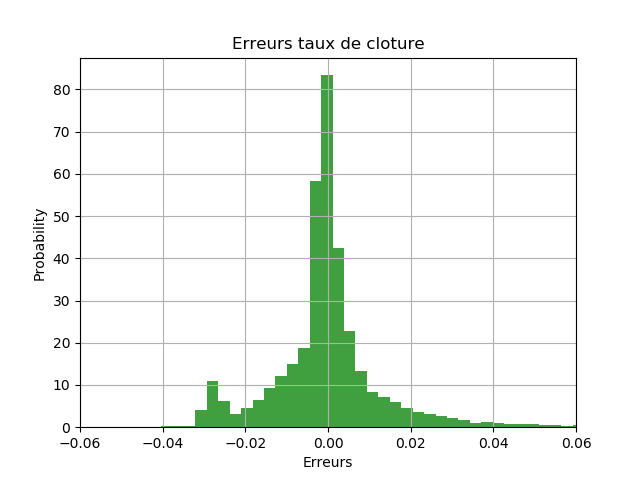
\includegraphics[height=10cm,width=16cm]{E_cloture.png}
%\caption{Nappe, taux versement }
\end{figure}

Le tableau \ref{loi_erreurs} contient quelques statistiques décrivant la loi de probabilité des erreurs. Notez que la moyenne est presque nulle. C'est quelque chose qui devrait normalement se produire.
On peut simuler une variable aléatoire avec la loi des erreurs. Pour cela, il suffit de savoir que si $I$ est un nombre entier $SI$, uniformément compris entre $1$ et $T$, donc,  
$E_I$
est une variable aléatoire avec la loi empirique des erreurs.



\begin{table}[h!]
	\caption{Loi des erreurs, taux de clôture.}
	\bigskip	
	\label{loi_erreurs}
	\centering
	\csvautotabular{percentile_erreurs.csv}
\end{table}


\subsection{Modèle sans caractéristiques individuelles de contrats}

Dans cette section, on va étudier  l'effet de négliger les caractéristiques individuelles des contrats des plan d'épargne logement, a savoir, les variables {\it Montant souhaité} et {\it Durée Souhaité}, sur la considération d'encours agrégés par génération mensuelle de production.  

On a besoin de isoler l'effet de utiliser l'estimateur de Nadaraya-Watson, car il produit lui-même une erreur d'estimation. Une autre erreur est produite par les variables non observables, c'est-à-dire celles qui ont été modélisées par des variables aléatoires indépendantes dans la construction de la base de données, ou théoriquement, la variable $ \varepsilon$ dans l'équation $$Y = f(X) + \varepsilon.$$

Afin d'éliminer les variables {\it Montant souhaité} et {\it Durée Souhaité} et se concentrer uniquement dans l'estimateur de Nadaraya-Watson, on reconstruit a nouveau la base de données "Stock\_Pel" mais cette fois-ci, avec de épargnantes homogènes: avec les même caractéristiques individuelles, a savoir, les moyennes correspondante a la base  "Stock\_Pel":

\begin{description}
\item {\it Montant souhaité} = 35000 $(=(10000 + 60000)/2)$ et
\item {\it Durée souhaité} =84 $(= 7 ans = (4 + 10)/2.$
\end{description}

On utilise la même régression non paramétrique, avec le même noyau

$$K(x)= e^{-\|x\|^2}$$

et la même fenêtre de lissage

$$ H=diag(h_1,h_2) \mbox{ avec $h_1=$ 1 mois et $h_2=$ 2\%}. $$

Dans ce cas, le coefficient de détermination $R^2$ pour le taux de clôture est égale a 
$$R^2 = 0.82\% $$
et pour le taux de versement
$$ R^2 = 0.98 \%$$

Les mêmes raisons qui expliquent le $R^2$ de $98\%$ dans la page \pageref{aqui}, nous font comprendre pourquoi il n'y a pas de changement dans la qualité du modèle pour le taux de versements.

Pour le taux de clôture, le $R^2$ passe de $0.59\%$ a $0.82\%$. On peut espérer donc de gagner 59/82 = 30\% de performance avec un modèle que prendre en considération l'effet des caractéristiques individuels de contrats. 

Le l'objectif n'est pas de quantifier la perte en performance, mais simplement de justifier que le fait d'agréger les contrat PEL  par génération, néglige  un certain nombre d'effets que peut avoir un impact significative dans l'estimation des taux de clôture et de versement.  

\section{Conclusions}

Nous avons créé une base de données appelée \\{\it Stock\_Pel} qui contient des informations mensuelles sur les clôtures et les versements de la phase d'épargne des Plans d'Épargne Logement ouverts entre janvier 1999 et août 2019. La base a été construite en tenant compte des caractéristiques propres de chaque PEL et elles ne sont plus observables lors de l'agrégation des encours par strates mensuelles. 

Nous avons étudié la performance sur notre base de la méthode de régression non paramétrique avec noyau de Nadaraya-Watson exponentiel avec deux variables explicatives : le taux du marché et l'âge du PEL. Nous avons choisi la fenêtre de lissage en séparant la base en deux parties, une "train data" pour calibrer et une "test data" pour tester le modèle. La fenêtre de lissage la plus performante est $h_1 = 1$ mois pour la variable explicative "âge" et $h_2 = 2\%$  pour la variable explicative "écart de taux". 

Le coefficient de corrélation du taux de marché (représenté par l'écart de taux euribor 3m et le taux PEL de la phase épargne) est de $0.2$ avec le taux de versement et de $-0.15$ avec le taux de clôture. Les deux coefficients sont bas, mais nous ne pouvons exclure le marché en tant que variable explicative. La première raison est que nous sommes dans une période où les taux d'intérêt sont très bas et donc peu variables, ce qui se traduit par des coefficients de corrélation historiques faibles.

La deuxième raison est que le CNC demande dans son avis \cite{CNC1} de modéliser le comportement des épargnants face aux fluctuations du taux de marché.

Les modèles ont été comparés par rapport à leur coefficient de détermination pour la "test data", dénoté $R^2$. Pour le taux de clôture, on obtient un $R^2 = 60\%$ et pour le taux de versements, un $R^2 = 0.98\%$. Le dernier est assez élevé parce que la base a été construite de manière à ce que les variables individuelles de chaque PEL ont très peu d'impact sur les décisions de versements de chaque client. En plus, elles sont diluées lorsque l'on ajoute un grand nombre d'observations, ceci grâce à la loi des grands nombres.

Nous avons fait une analyse des résidus de la régression non paramétrique pour le taux de clôture afin de pouvoir estimer sa loi de probabilité. Cette loi peut être remplacée par une approximation donnée par la loi empirique représentée par l'histogramme \ref{E_cloture}. La loi est assez symétrique et très concentrée autour de $0$. Cette dernière nous donne un aspect positif de la régression.

Nous avons étudié l'effet de la non prise en compte des caractéristiques individuelles des contrats des plans d'épargne logement sur la considération des encours agrégés par génération mensuelle de production.  Afin d'isoler l'effet de l'estimation de Nadaraya-Watson, car elle produit aussi une erreur d'estimation, nous avons reconstruit à nouveau la base de données  mais cette fois-ci, avec des PEL homogènes où les caractéristiques individuelles ne sont plus présentes. 

Pour le taux de clôture, le $R^2$ passe de $0.59\%$ à $0.82\%$. On peut espérer donc gagner $59/82 = 30\%$ de performance avec un modèle qui prend en considération l'effet des caractéristiques individuelles de contrats. L'objectif n'était pas de quantifier la perte en performance, mais simplement de justifier que le fait d'agréger les contrat PEL par génération néglige un certain nombre d'effets qui peuvent avoir un impact significatif dans l'estimation des taux de clôture et de versement.  
 
\chapter{Calcul de la provision épargne}
\label{chap2}
\section{Introduction}
Au chapitre \ref{chap1}, nous avons déterminé un modèle comportemental pour les plans d'épargne logement qui tient compte de la variable déterministe "âge" du PEL, et la variable aléatoire donnée par l'écart entre le taux du PEL de la phase épargne et le taux du marché Euribor à 3 mois. Ainsi, les taux sur le marché jouent un rôle crucial dans la détermination des encours futurs des plans d'épargne logement et donc dans le calcul de la provision. L'avis \cite{CNC1} mentionne que les encours futurs d'épargne  dépend du niveau futur des taux et des comportements des épargnants dans différents contextes possibles de taux.

Les taux du marché sont également déterminants pour le calcul d'autres composantes de la provision : le taux de référence et les facteurs d'actualisation. Les engagements doivent être mesurés par référence aux taux offerts à la clientèle particulière, en cohérence avec la durée de vie estimée des encours et leur date de mise en place. Les pertes futures résultant de rémunérations pré-fixées par la réglementation (donc, hors marché), sont évaluées par rapport aux rémunérations que percevrait l'établissement sur des produits financiers présentant des caractéristiques similaires, mais dont la rémunération est fixée par le jeu des forces de marché. Les pertes correspondent pour l'établissement au coût de distribution d'instruments financiers hors marché. \cite{CNC2}.

La provision se calcule en valeur actuelle. L'avis \cite{CNC1} précise que le taux d'actualisation retenu doit être déduit de la courbe Euribor 3 mois à la date d’évaluation, et moyenné sur une période de douze mois. Cette dernière disposition permet de prendre en compte la durée de vie longue de ces produits d'épargne et de crédit et d'éliminer l'effet des fluctuations erratiques à court terme des taux sur l'évaluation, tout en intégrant l'effet des tendances fondamentales des taux.

Par conséquent, pour le calcul de la provision épargne logement, nous devons modéliser différents taux de marché à différentes maturités : par exemple le taux Euribor 3 mois et le taux des obligations assimilables d'État OAT à 10 ans, ainsi que les corrélations entre eux.

Dans ce contexte, les modèles de taux à un facteur, comme par example le modèle de taux de Vasicek, ne peuvent pas être utilisés en raison de leurs limites en ce qui concerne la modélisation des corrélations entre taux de différentes maturations (Voir Brigo et Mercurio \cite{BM}). Nous devons utiliser des modèles de taux multifactoriels.

Dans la section \ref{SmodeleTaux} nous allons introduire le modèle à deux facteurs $G2++$ ainsi que des formules fermées pour calculer le prix des obligations zéro coupon et les taux d'intérêt de différentes maturités.

Dans la section \ref{calibration}, nous présentons un résultat qui nous permet de calibrer les paramètres du modèle à partir des observations historiques des taux d'intérêt. Cette méthode diffère de celle présentée au chapitre 4 de Brigo et Mercury \cite{BM}, basée sur le prix des produits financiers observés à un instant donné et donc dans un contexte de probabilité risque neutre. Les paramètres du modèle $G2++$ seront calibrés en fonction de l'historique mensuel des taux Euribor à 3 mois et OAT à 10 ans.

La modélisation des taux d'intérêt nous permet d'estimer les encours futurs et la provision pour le plan d'épargne logement. Cette dernière est une variable aléatoire qui dépend de l'incertitude des taux du marché. A l'aide des simulations de Monte Carlo, nous obtenons une estimation de sa loi de probabilité. Son espérance sera la mesure utilisée pour déterminer la provision d'un point de vue comptable. 

Nous suivrons l'étude que nous avons commencée au chapitre \ref{chap1} et qui concerne l'effet de l'agrégation  des comptes par mois de production, en éliminant l'effet des variables propres à chaque compte individuel. Dans le chapitre \ref{chap1}, nous avons vu que cela implique une perte de la performance du modèle comportemental. Ici nous verrons l'effet que cela aura sur le montant de la provision.

Enfin, nous allons mesurer l'effet sur le calcul de la provision que pourrait avoir l'incorporation de nouvelles variables explicatives, sur la base de la modélisation des résidus de la régression non paramétrique effectuée au chapitre \ref{chap1}.

\section{Le modèle de Taux}
\label{SmodeleTaux}
Cette section est basée sur le chapitre 4 du livre de Brigo et Mercurio \cite{BM}. Nous présentons le modèle de taux courts à deux facteurs a utiliser pour le calcul de la provision. D'abord, on va motiver les modèles à deux facteurs en soulignant les faiblesses des modèles à un facteur. Avec le taux court ou taux instantanée $r_t$ on peut calculer le prix des obligations zero coupon à partir de la relation 

$$ P(t,T) = E_t \left[ exp\left( -\int_t^T r_s ds \right)\right]$$

Par exemple pour le modèle de taux de Vasicek avec paramètres de drift $(\theta, k)$, volatilité $\sigma$ et source d'incertitude donnée par un mouvement Brownien $(W_t)$: 

$$ dr_t = k(\theta -r_t)dt +\sigma dW_t,$$
il y a des fonctions $A(t,T)$ et $B(t,T)$ telles que
$$P(t,T) = A(t,T)exp(-B(t,T)r_t.$$
Le taux zero coupon ou instantanée est de la forme
$$R(t,T) := -\frac{1}{T_t}log P(t,T)= a(t,T)+b(t,T)r_t.$$
Avec le modèle de Vasicek, la corrélation entre deux taux zero coupon $R(t,T_1)$ et $R(t,T_2)$
$$Corr(R(t,T_1), R(t,T_2) = 1,$$
A tout moment, les taux d'intérêt de différentes maturités sont parfaitement corrélés, qui diffère de ce qui est observé sur le marché.

Dans le calcul de la provision, on utilise différentes maturités de taux, par example, le taux euribor 3 mois pour les calcul de facteurs d'actualisation, des taux a maturités supérieur a 5 ans pour le calcul de taux de référence. C'est très importante de pouvoir prendre en compte la corrélation observée.

La corrélation joue un rôle pertinent, nous devons passer à un modèle permettant obtenir des corrélations entre les taux de différentes maturités plus réalistes. C'est la nécessité d'utiliser les modèles a deux facteurs :

\begin{eqnarray}
r_t &=& x_t + y_t\nonumber\\
dx_t &=& -ax_td_t +\sigma dW_t^1\nonumber\\
dy_t &=& -by_t dt +\eta (\rho dW_t^1 +\sqrt{1-\rho ^2}d W_t^2) \nonumber
\end{eqnarray}

Le prix d'une obligation zero coupon a l'instante $t$ de maturité a la date $T$ est donné par la formule
\begin{eqnarray}
P^M(t,T) &=&\frac{P^M(0,T)}{P^M(0,t)}exp(A(t,T))\label{PtT}\\ 
A(t,T) &=& \frac{1}{2}[V(T-t)-V(T)+V(t)] \nonumber\\
	   & & -B(a, T-t)x_t  -B(b,T-t)y_t\nonumber
\end{eqnarray}
avec les fonctions $V$ et $B$ définie par:

\begin{eqnarray}
V(t)&=&\frac{\sigma^2}{a^2}\left[ t+B(2a,t)-2B(a,t)\right]\nonumber\\
& &+\frac{\eta^2}{b^2}\left[ t+B(2b,t)-2B(b,t)\right]\nonumber\\
& &+2\rho\frac{\sigma\eta}{ab}\left[ t+B(a+b,t)-B(a,t)-B(b,t)\right]\label{Vt}
\end{eqnarray}
et $B$ définie par
\begin{equation}
\label{B(z,t)}
B(z,t) := \frac{1-e^{-zt}}{z}.
\end{equation}
Le suffixe $M$ dans la formule (\ref{PtT}) serve a dénoter la curve zero coupon initial $P^M(0,t), t\geq 0$. Par example, $P^M$ peut être la courbe zero coupon Euribor où la courbe zero coupon des obligations d'état OAT.
Le taux d'intérêt instantané ou taux zero coupon est donné par $R^M(t,T)$ définie par
\begin{equation}
\label{RtT}
R^M(t,T) = -\frac{\log(P^M(t,T))}{T-t},
\end{equation}
c'est le taux continue constant sur la période $[t,T]$ tel que
$$ P^M(t,T) = \exp(-R^M(t,T)(T-t) ) $$

\section{Calibration du modèle $G2++$}
\label{calibration}
Dans le modèle $G2++$, le taux instantanée est définie par le processus
$$ r_t = x_t + y_t +\varphi (t) $$
ou $\varphi$ est une fonction déterministe et elle est utilisé pour ajuster le modèle à la courbe de taux zero coupon initial. Le processus $(x_t, y_t)$ est un processus d'Ornstein-Uhlenbeck

\begin{eqnarray}
dx_t &=& -ax_td_t +\sigma dW_t^1\nonumber\\
dy_t &=& -by_t dt +\eta (\rho dW_t^1 +\sqrt{1-\rho ^2}d W_t^2) \nonumber
\end{eqnarray}
où $W^1$ et $W^2$ sont deux mouvements Browniens standard et indépendantes. Le paramètre $\rho$ est un coefficient de corrélation, c'est à dire $-1\leq \rho \leq 1$. La solution aux equations différentielles stochastiques précédentes sont donnée par :
\begin{eqnarray}
x_t &=& x_s e^{-a(t-s)} +\sigma \int_s^t e^{-a(t-u)}dW^1_u\label{x_t}\\
y_t &=& y_s e^{-b(t-s)} +\eta\rho \int_s^t e^{-b(t-u)}dW^1_u+\eta\sqrt{1-\rho ^2}\int_s^t e^{-b(t-u)}dW^2_u\label{y_t}
\end{eqnarray}

L'outil que nous utiliserons pour calibrer le modèle est la proposition suivant qui nous permet d'utiliser les données historiques des différents taux d'intérêt. Nous supposons que nous avons l'historique par périodes mensuelles. Dénote par $R^i(n)$ le taux zero coupon ou mois $n$ de maturité $T^i$ et lié à la structure des taux d'intérêt des facteurs d'actualisation $t\rightarrow P^{M^i}(0,t)$. Par example, $R^1(n)$ peut être le taux Euribor a 3 mois ou mois $n$, $R^2(n)$ le taux à 10 ans de la courbe OAT des obligations assimilables de trésor, etc. 

De (\ref{RtT}) et (\ref{PtT}) nous avons :
\begin{eqnarray}
T^i R^i(n)&=&-\log P^{M^i}(0,T^i+n/12)+\log P^{M^i}(0,n/12)\nonumber\\
&&-\frac{1}{2}\left[ V(T^i)-V(T^i+n/12)+V(n/12)\right]\nonumber\\
&&+B(a,T^i)x_{n/12}+B(b,T^i)y_{n/12}.\nonumber
\end{eqnarray}  

\begin{prop}
\label{CONV_LIMIT}
Si les courbes zero coupon satisfont l'hypothèse
$$\frac{P^{M^i}(0,T^i + n/12)}{P^{M^i}(0,n/12)}\mbox{ converge lorque }n\rightarrow \infty,$$
alors,
\begin{eqnarray}
& &\lim_{N\rightarrow \infty}\widehat{Cov}_N(i,j)\nonumber\\
&:= &\lim_{N\rightarrow \infty} \frac{1}{N}\sum_{n=1}^N \left[R^i(n+1)-R^i(n)\right]\left[ R^j(n+1)-R^j(n)\right]\nonumber\\
&=&\sigma^2 B(a,1/12)\frac{B(a,T^i)B(a,T^j)}{T^iT^j}\nonumber\\
& &+\eta^2 B(b,1/12)\frac{B(b,T^i)B(b,T^j)}{T^iT^j}\nonumber\\
& &+\frac{\rho\sigma\eta}{a+b}[aB(a,1/12)+bB(b,1/12)]\nonumber\\
&&\mbox{ }\times\left[\frac{B(a,T^i)B(b,T^j)}{T^iT^j}+\frac{B(a,T^j)B(b,T^i)}{T^iT^j}\right]\nonumber
\end{eqnarray}

\end{prop}

Le pre-limit $\widehat{Cov}_N(i,j)$ est un estimateur de la covariance entre le deux taux $R^i$ et $R^j$.
On dénote par $Cov$,la limite de la proposition précédente par $Cov$, c'est a dire :
$$Cov(i, j) = \lim_{N\rightarrow infty} \widehat{Cov}_N(i,j)$$
qui est une fonction du paramètres
$$(a, b, \sigma, \eta, \rho) \rightarrow Cov(i,j).$$

 La preuve sera donne dans la dernier section du présent chapitre. A titre d'exemple, avec les paramètres de la section 4.2.7 de Brigo et Mercurio \cite{BM} : 
$$a = 0.77, b = 0.082, \sigma = 0.02, \eta= 0.01 \mbox{ and }\rho = -0.7,$$
on a simulé,  avec le programme python gpp.py de l'annexe \ref{gpp.py}, 10 trajectoires de 120 mois de taux zero coupon de maturité 3 et 12 mois et émis a partir de la courbe OAT de juillet 2019. 

La courbe OAT utilisé est présenté dans le graphique \ref{courbeOAT} est elle est calculé a partir des données de la Banque de France et interpolés par la méthode de splines cubiques.  

Pour chaque trajectoire, les valeurs des estimateurs sont présentés dans le tableau \ref{estimateurs} ci-dessous, en termes de pourcentages de son valeur de convergence théorique $Cov(i, j)$:
 $$Cov(i, j) = lim_{N\rightarrow \infty}\widehat{Cov}_N(i,j) = 1.066 \times 10^{-5}.$$

\begin{table}[h!]	
	\caption{
	\bf Valeurs des estimateurs en \%.}
	\bigskip	
	\label{estimateurs}
	\centering
	\csvautotabular{estimateurs.csv}
\end{table}


\subsubsection{Exemple de calibration.}
Nous verrons après,  que pour calculer la provision, nous aurons besoin du taux Euribor 3 mois pour les facteurs d'actualisation et le comportement des épargnants et du taux OAT 10 ans comme proxi pour le taux de référence. On peut essayer de calibrer le modèle G2++ avec les donnes historiques de taux que nous venons de mentionner, mais la différence entre les tailles des maturités 10 ans et 0.25 ans peut causer des problèmes d'estimation. Pour éviter ce problem, on va utiliser a la place l'historique de taux Euribor à 1 an en la taux OAT a 5 ans, qui sont tout à fait liées respectivement aux premières. 

Avec la notation de la section précédente :
$$R^1:=\mbox{ Taux Euribor a 1 an et,}$$
$$R^2:=\mbox{Taux OAT 5 ans} $$

Nous avons l'historique à 10 ans, donc $N = 120$. La covariance observé $\widehat{Cov}_N(i, j)$, $1\leq i,j \leq 2$ est donné par :

$$
\widehat{Cov}_N = \left(
\begin{array}{cc}
3.3 \times 10^{-7} & 2.67 \times 10^{-7}\\
2.67 \times 10^{-7} & 2.71 \times 10^{-6}
\end{array}
\right)
$$

On a cherché les paramètres $$\mathcal{P} = (a, b, \sigma, \eta,\rho )$$ de manière à ce que
la différence entre $\widehat{Cov}_N$ et $Cov(\mathcal{P})$ soit minimal dans le sens ou

$$ \varphi(\mathcal{P}) :=  \sum_{i=1}^2\sum_{j=1}^2 \left( Cov(\mathcal{P}(i, j)/\widehat{Cov}_N(i, j) - 1  \right)^2$$
soit minimal. 

On obtient les paramétrés avec le problème d'optimisation 
$$\min_{\mathcal{P}}\varphi(\mathcal{P}).$$

En tenant compte du fait que les matrices $Cov$ et $\widehat{Cov}_N$ sont symétriques, nous avons 3 fonctions à optimiser et 5 paramètres, on peut penser qu'il est possible de reproduire la matrice $\widehat{Cov}_N$ exactement, c'est-à-dire, trouver des paramètres $\mathcal{P}$ pour que la fonction $\varphi$ soit $0$. Cependant, les paramètres ont des restrictions qui éliminent la possibilité d'atteindre $\varphi(\mathcal{P}) = 0$. Par example, comme $\rho$ est le coefficient de corrélation entre les Browniens $W^1$ et $W^2$ nous avons $-1 \leq \rho \leq 1$ et d'après la section 4.2.3 de \cite{BM}, on doit avoir
$$-1\leq \rho < 0.$$
Pour avoir l'ergodicité des processus $x_t$ et $y_t$ nous avons besoins de
$$ a, b >0.$$
Finalement, $\sigma$ et $\eta$ sont des écarts-types et ils doivent donc satisfaire
$$ \sigma, \eta > 0.$$

Pour trouver les paramétrés qui minimisent la fonction $\varphi$ on a choisi entre une série généré aléatoirement. On a vu des minimums locaux possibles avec $\rho \sim -1$ que nous avons décidé de ne pas prendre en compte.

On a trouvé les valeurs suivantes des paramètres à estimer :
$$a = 1.6, b=0.06, \sigma=0.005, \eta=0.003, \rho=-0.73$$

La matrice $Cov$ avec les paramètres précédentes, est égale a

$$
Cov = \left(
\begin{array}{cc}
3.7 \times 10^{-7} & 2.7 \times 10^{-7}\\
2.7 \times 10^{-7} & 4.02 \times 10^{-7}
\end{array}
\right)
$$

qui, en termes de pourcentage par rapport a la matrice La matrice $\widehat{Cov}_N$ est égale a 

$$
\left(
\begin{array}{cc}
111\% & 101\%\\
101\% & 14\%
\end{array}
\right)
$$

Les paramètres ne reproduisent pas très bien, $\widehat{Cov}_N(2,2)$, qui est la variance du taux OAT a 5 ans. Il existe d'autres minima locaux possibles qui sont mieux adaptés à $\widehat{Cov}_N(2,2)$  mais qui s'écartent de $\widehat{Cov}_N(1,2)$, la covariance entre le taux Euribor 1 an et le taux OAT 5 ans. Pour nous, il est plus important de reproduire les covariances des taux. 


Une solution pour reproduire la matrice $\widehat{Cov}_N$ de manière plus précise s'est de introduire an troisième facteur $z_t$ dans le modèle et donc travailler avec un modèle $G3++.$

\section{Calcul de la provision.}

Les plan d'épargne logement contiennent différentes clauses qui, dans certaines configurations de taux intérêt, peuvent entraîner des pertes pour les établissements financières. L'avis du CNC \cite{CNC1} prévoit que les engagements aux conséquences défavorables pour les établissements doivent être provisionnés. Les engagements sont relatifs, d'une part, à l'obligation de rémunérer l'épargne dans le futur à un taux fixé à l'ouverture du contrat pour une durée indéterminée, et, d'autre part, à l'octroi d'un crédit aux souscripteurs à un taux déterminé fixé à l'ouverture du contrat.
Ces provisions doivent être calculées par génération de plans d'épargne-logement sachant qu'il n'y a pas de compensation possible entre les engagements relatifs à des générations différentes. Une génération de contrats se définit comme un ensemble de contrats partageant les mêmes caractéristiques réglementaires et, notamment, les mêmes conditions de taux pour les phases épargne et crédit. Jusqu'au présente, il y a 12 générations de PEL résumés dans le tableau \ref{taux_pel} de l'annexe \ref{app_pel}.

L'avis \cite{CNC1} mentionne que les encours futurs d'épargne et de crédit dépendent du niveau futur des
taux et des comportements des épargnants dans des différents contextes possibles de taux. Dans le chapitre \ref{chap1}, nous avons  estimé les comportements futurs des épargnantes avec une régression non paramétrique qui dépende de deux variables : 
\begin{center}
{\it L'écart} : ( taux euribor 3 mois - taux pel ) et {\it l'age} du Pel
\end{center}
Les paramètres du modèle des comportements ont été calculés a partir d'observations historiques de une longue période de plus de 20 ans. 

Puisque l'âge est une variable déterministe, on peut utiliser le modèle de taux $G2++$ calibré précédemment et les taux d'intérêt observables sur le marché comme base pour estimer les taux futures afin de déterminer différentes chemins "probables"  des montant des encours. 

Précisément, on a, a la date de juillet 2019, les taux euribor a différentes maturités .\footnote{https://fr.global-rates.com/taux-de-interets/euribor/2019.aspx} : 1 semaine, et 1, 3, 6 et 12 mois. Les taux sont présentés dans le tableau \ref{euribor_juillet} suivante.

\begin{table}[h!]
	\caption{\bf Taux Euribor, juillet 2019.}
	\bigskip	
	\label{euribor_juillet}
	\centering
	\csvautotabular{euribor_juillet.csv}
\end{table}

Avec une méthode de "splines cubiques": interpolation par morceaux avec des polynômes de degré 3 on peut obtenir les taux euribor pour toutes les maturités $T>0$ au juillet 2019 :
$$T \rightarrow \varphi_{eur}(T) $$

 Pour cela on a utilisé la function {\it interp1d} de la librairie python {\it scipy.interpolate}. On obtient la fonction représenté dans le graphique \ref{courbeEuribor} suivante.


\begin{figure}[!h]
\label{courbeEuribor}
\centering
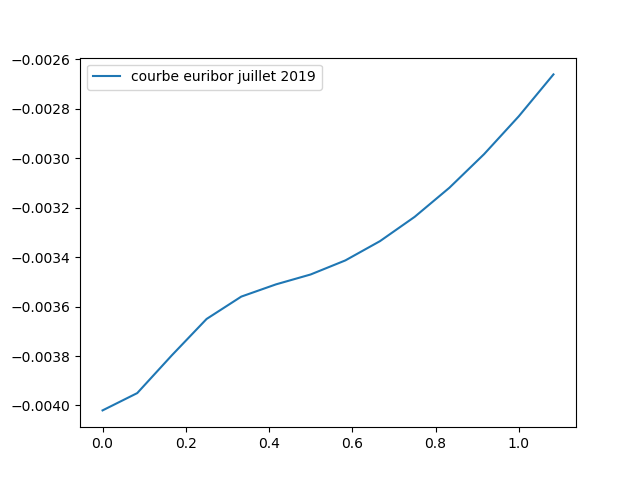
\includegraphics[height=10cm,width=16cm]{courbeEuribor.png}
\caption{Courbe Euribor juillet 2019}
\end{figure}

Soit $(x_t, y_t)$ le modèle  $G2++$ (\ref{x_t}) et (\ref{y_t} avec les paramètres trouvés dans la section précédente :
\begin{equation}\label{parametros}
a = 1.6, b=0.06, \sigma=0.005, \eta=0.003 \mbox{ et } \rho=-0.73
\end{equation}

Le taux Euribor à maturité $T =1/4$ (3 mois) à la date $t$ est donné par :
\begin{eqnarray}
\tau_{t/12} &=& 4\left( \varphi_{eur}(1/4+t)-\varphi_{eur}(t)\right.\nonumber\\
& &-0.5(V(1/4)-V(1/4+t)+V(t))\nonumber\\
& &\left.+B(a, 1/4)x_t + B(b, 1/4)y_t\right)\label{t_euribor}
\end{eqnarray}
où les fonctions $V$ et $B$ sont données respectivement par (\ref{Vt}) et (\ref{B(z,t)}). On a utilisé $\tau_{t/12}$ à la place de $\tau_t$ dans l'équation précédente pour simplifier la notation lorsqu'on travaille avec des données mensuelles : Le taux Euribor 3 mois ou mois $n$ est $\tau_n$.

On a trouvé dans le chapitre \ref{chap1}, des fonctions :
$$ \Tc(age, ecart\_taux)\mbox{ et }\Tv(age, ecart\_taux)$$
qui associent à chaque PEL d'âge {\it 'age'} avec un scénario de taux représenté par {\it 'ecart\_taux'}, les taux de clôture et de versements.

Soit $\E_n$ la somme agrégée, au mois $n$,  de tous les PEL ouverts il y a $a$ mois (les pel sont âgés de $a$ mois). Soit $\tau_{pel}$ le taux épargne associé au PEL. L'encours d'aujourd'hui $\E_0$ est observé et pour les mois suivants $n\geq 1$, on obtient récursivement :
\begin{equation}\label{En}
\E_n = \E_{n-1}\left( 1 + \Tv(a + n-1,\tau_{n-1}-\tau_{pel})-\Tc(a + n-1,\tau_{n-1}-\tau_{pel}) \right).
\end{equation}


L'incertitude sur le niveau de l'encours futur et son évolution dans le temps est notamment due au niveau des taux du marché, particulièrement, du processus aléatoire :
$$ \omega \rightarrow (\tau_n(\omega)).$$
L'incertitude est donc représentée par l'espace de probabilité $(\Omega,\mathcal{F})$ et la mesure de probabilité du Mouvement Brownien bidimensionnel $(W^1,W^2)$ définie en (\ref{x_t}) et(\ref{y_t}). 

{\it L'encours minimum} ou {\it certain} est défini comme celui qui sera dans n'importe quel scénario de taux d'intérêt \cite{CNC2}. Pour chaque mois $n$, l'encours certain est donné par
\begin{equation}\label{Ec}
\E_n^c = \min_{\omega \in \Omega} \E_n(\omega).
\end{equation}
Notez que l'encours certain est déterministe et normalement, il doit être positive au mois pour les premier mois $n$. En fait, si le taux de rémunération du Pel est plus important que les taux du marché, les encours ont tendance à être élevé . Au contraire, si le taux du Pel est faible par rapport au taux du marché, les propriétaires des Pel, vont épargner afin d'avoir un taux de prêt avantageux dans l'avenir. 

L'encours certain peut être évalué statistiquement sous un intervalle de confiance très élevé \cite{CNC2}, c'est a dire, en lieu du minimum en (\ref{Ec}), on peut utiliser le quantile a 97.5 \% et il ne diffère pas, au plan comptable, d'un portefeuille de dépôts à terme, n'ayant aucun caractère optionnel. Il doit en conséquence demeurer comptabilisé à la valeur nominale de ses constituants. 

La fraction de l'encours incertain qui génère un risque est dite "encours d'épargne en risque" et, pour chaque période future, il est estimé par différence entre les encours d'épargne probables et les encours d'épargne minimum attendus:

$$ \E_n^{risque} := \E_n -\E_n^c,$$
et c'est le seule montant auquel une provision doit être ajoutée.
\begin{figure}[!h]
\label{surface_risque}
\centering
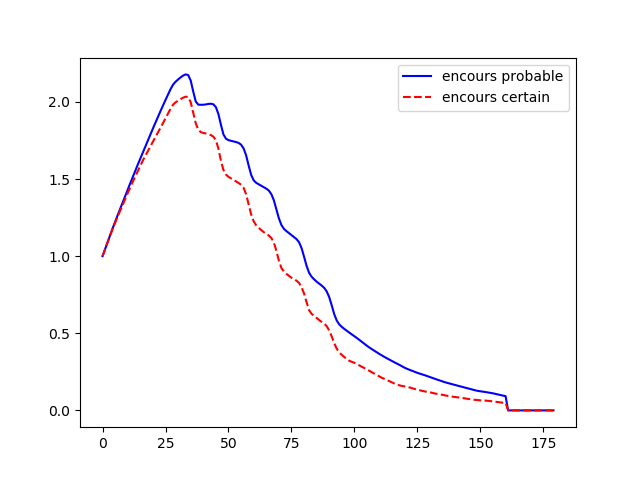
\includegraphics[height=10cm,width=16cm]{surface_risque.png}
\caption{Encours en risque.}
\end{figure}

Les engagements doivent être mesurés par référence aux taux offerts à la clientèle particulière, en cohérence avec la durée de vie estimée des encours et leur date de mise en place. Les pertes futures résultant de rémunérations pré-fixées par la réglementation (donc, hors marché), sont évaluées par rapport aux rémunérations que percevrait l'établissement sur des produits financiers présentant des caractéristiques similaires, mais dont la rémunération est fixée par le jeu des forces de marché. Les pertes correspondent pour l'établissement au coût de distribution d'instruments financiers hors marché. \cite{CNC2}.


Pour les engagements sur la phase épargne des plans d'épargne-logement, les {\it taux de référence} sont notamment les taux des dépôts à terme, des obligations ou des produits d'assurance-vie. La difficulté du choix réside dans le fait que aucun instrument financier d'épargne existant ne reproduit  strictement les caractéristiques des plans d'épargne-logement. Néanmoins, le produit d'épargne de référence choisi doit rester le même dans le temps pour un même établissement. \cite{CNC2}.

Si on dénote par $\tau_{ref}$ le taux de référence choisi, il doit dépendre des conditions de "marché", c'est à dire, il dépend des niveaux de taux : $\tau_{ref} = \tau_{ref}(\omega)$.

Pour un mois donné $n$, l'établissement financière rémunère le propriétaires du pel au taux $\tau_{pel}$ malgré le fait que, compte tenu des conditions du marché, il devrait rémunérer au taux $\tau_{ref}$. 

Les résultats futurs sur les encours en risque peuvent être estimés en multipliant le montant de
ces encours par la différence entre $\tau_{pel}$ et $\tau_{ref}$. Pour l'établissement financière, la perte au mois $n$, est :
$$\frac{1}{12}(\E_n(\omega) - \E_n^c)(\tau_{pel} - \tau_{ref}(\omega)),$$
(c'est un gain pour l'établissement financier si ce dernier est négative). Le facteur $1/12$  apparaît parce que les taux $\tau_{pel}$ et $\tau_{ref}$ sont annuels et doit calculer la perte pour le mois $n$ uniquement.

Les taux de référence sur la phase épargne suggères dans  l'avis \cite{CNC1} sont très corrélés avec le taux des obligations assimilables d'état a 10 ans. Le taux de référencé peut être calculé a a partir des donnes historiques du taux OAT 10 ans. Pour simplifier, nous avons  décidé de prendre ce dernier comme taux de référence :
$$ \tau_{ref} = \mbox{ taux OAT 10 ans}.$$

Le taux de référence, donc le taux OAT 10 ans est calculé de la même manière que le taux Euribor 3 mois. Précisément, on a, a la date de juillet 2019, les taux OAT a différentes maturités, pris du site de la Banque de France\footnote{https://www.banque-france.fr/statistiques/taux-et-cours/taux-indicatifs-des-bons-du-tresor-et-oat}: 1, 3, 6, 9 mois et 1, 2, 5, 10 et 30 ans. Les taux sont présentés dans le tableau \ref{oat_juillet} suivante.

\begin{table}[h!]
	\caption{\bf Taux OAT, juillet 2019.}
	\bigskip	
	\label{oat_juillet}
	\centering
	\csvautotabular{oat_juillet.csv}
\end{table}

Avec la méthode de "splines cubiques" (function {\it interp1d} de la librairie python {\it scipy.interpolate}) on obtient les taux OAT pour toutes les maturités $T>0$ au juillet 2019 :
$$T \rightarrow \varphi_{oat}(T),$$
représenté dans le graphique \ref{courbeEuribor} suivante.


\begin{figure}[!h]
\label{courbeOAT}
\centering
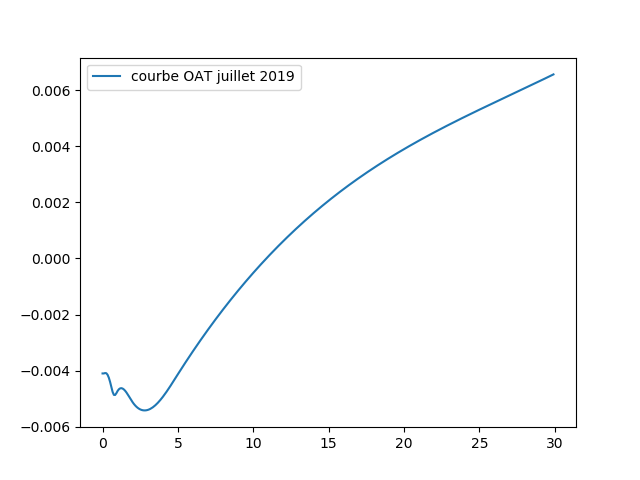
\includegraphics[height=10cm,width=16cm]{courbeOAT.png}
\caption{Courbe OAT juillet 2019}
\end{figure}

Le taux OAT a maturité $T =10$ a la date $t$ est donné par :
\begin{eqnarray}
\tau_{ref}(t/12) &=& 4\left( \varphi_{oat}(10+t)-\varphi_{oat}(t)\right.\nonumber\\
& &-0.5(V(10)-V(10+t)+V(t))\nonumber\\
& &\left.+B(a, 10)x_t + B(b, 10)y_t\right)\label{t_oat}
\end{eqnarray}
ou les fonctions $V$ et $B$ sont donnés respectivement par (\ref{Vt}) et (\ref{B(z,t)}). Le taux OAT 10 ans ou mois $n$ est $\tau_{ref}(n)$.

La provision se calcule en valeur actuelle. L'avis \cite{CNC1} précise que le taux d'actualisation retenu doit être déduit de la courbe Euribor 3 mois à la date d’évaluation, et moyenné sur une période de douze mois. Cette dernière disposition permet de prendre en compte la durée de vie longue de ces produits d'épargne et de crédit et d'éliminer l'effet des fluctuations erratiques à court terme des taux sur l'évaluation, tout en intégrant l'effet des tendances fondamentales des taux.

Dénotez par $\bar{\tau}_n$ le taux Euribor 3 mois, a la date $n$ et moyennée sur $12$ mois :
$$\bar{\tau}_n =\frac{1}{12}\sum_{i=n-11}^n \tau_n.$$
Le taux $\bar{\tau}_n$ est une version "régularisé" du $\tau_n$, comme le montre le graphique \ref{euribor3m_vs_moy_3m} ci-dessous.

\begin{figure}[!h]
\label{euribor3m_vs_moy_3m}
\centering
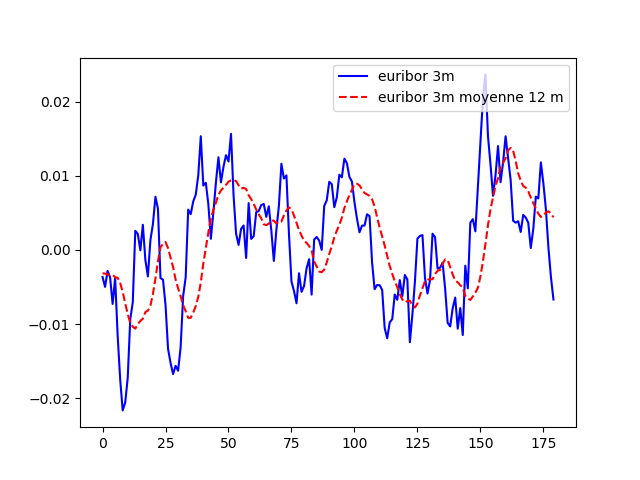
\includegraphics[height=10cm,width=16cm]{euribor3m_vs_moy_3m.png}
\end{figure}

Le facteur d'actualisation de mois $n$ au mois $n-1$, c'est à dire, le valeur au mois $n-1$ d'un euro au mois $n$ est donné par:
$$DF_{n-1,n} = DF_{n-1,n}(\omega) = \left(\frac{1}{1 + \bar{\tau}_{n-1}}\right)^{1/12}.$$
Le facteur d'actualisation est donné par $DF_0 = 1$ et pour $n\geq 1$:
$$DF_n = DF_n(\omega) = \prod_{j=0}^{n-1} \left(\frac{1}{1 + \bar{\tau}_{j}}\right)^{1/12}  $$

Pour l'établissement financière, la perte au mois $n$ actualisé, est :
$$\frac{1}{12}DF_n(\omega)(\E_n(\omega) - \E_n^c)(\tau_{pel} - \tau_{ref}(\omega)),$$
et montant total des pertes actualisés, si le scénario de taux $\omega$ se réalise est égale a:
\begin{equation}\label{perte}
perte(\omega)=\sum_{n=0}^{\infty}\frac{1}{12}DF_n(\omega)(\E_n(\omega) - \E_n^c)(\tau_{pel} - \tau_{ref}(\omega)).
\end{equation}

D'après le tableau \ref{taux_pel} dans l'annexe \ref{app_pel}, on a 5 générations de PEL, car on considère uniquement les PEL de mois de 15 ans, donc ouvert a partir de septembre 2004. Les générations sont  présentés dans le tableau \ref{generation_pel} ci-dessous.

\begin{table}[h!]
	\caption{\bf Générations de PEL ouverts a partir de septembre 2004.}
	\bigskip	
	\label{generation_pel}
	\centering
	\csvautotabular{generation_pel.csv}
\end{table}

N'oublions pas que la perte actualisé \ref{perte} a été calculé sur une {\it strate} des pel, c'est à dire, sur l'ensemble des pel ouverts a une mois en particulier. Si $\mathcal{S}$ est une {\it strate} des pel, on dénote sa perte actualisé par 
$$ perte_{\mathcal S}(\omega)$$
qui est donné par la somme (\ref{perte}) associé a la strate.

Pour chaque génération de PEL $\mathcal{G} \in \{8, 9, 10, 11, 12\}$ la provision est égale au maximum entre $0$ et la somme des pertes actualisés de toutes les {\it strates} qu'appartient à la génération, car s'il y a compensation possible entre des strates appartenant à la même génération. Mathématiquement, la provision pour la génération $\mathcal{G}$ est égale a
\begin{equation}
\label{provision_g}
provision_\mathcal{G}(\omega) = \max\left(0, \sum_{\mathcal{S}\in \mathcal{G}}perte_\mathcal{S}(\omega)\right)
\end{equation}
Comme il n'y a pas compensation possible entre les provisions de différentes générations, la provision est total est donné par
\begin{equation}
\label{provision}
provision(\omega)=\sum_{\mathcal{G}=8}^{12} provision_\mathcal{G}(\omega).
\end{equation}

Ici, on a travaillé uniquement avec les pertes actualisés sur la phase épargne du PEL. Normalement il faut ajouté les pertes actualisés de la phase crédit mais on a fait, pour simplifier, l'hypothèse que les pertes sur la phase crédit sont 0. Cette hypothèse est observable actuellement car les taux de marchés sont très bas, et donc il n'y pas de conversion de pel en crédit.

La provision est une variable aléatoire, elle dépende de l'incertitude $\omega$ lie au marché. Pour chaque scénario de taux possible, ou probable, on a une provision. Le montant d'argent a provisionner dépendra de l'appétence au risque de l'institution financière. Le plus acceptable est de prendre la espérance de la provision ou un de quantiles comme la médiane, ou le quantile a 60\%.

On a estimé la loi de probabilité de la provision avec 1000 simulations de Monte Carlo. On a simulé 1000 trajectoires du processus G2++ avec les paramètres (\ref{parametros}) précédemment estimés. Pour chaque trajectoire on a calculé la provision par génération (\ref{provision_g}) et la provision totale (\ref{provision}). L'ensemble de 1000 provisions forme ce que nous appelons la loi empirique et elle est représenté par le suivante histogramme.  

\begin{figure}[!h]
\label{loi_empirique}
\centering
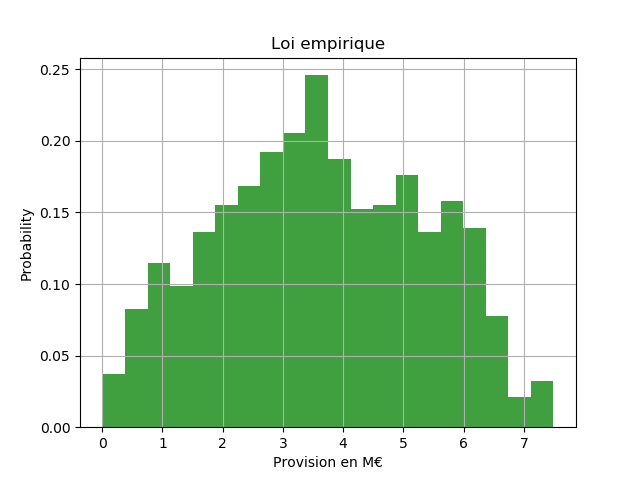
\includegraphics[height=10cm,width=16cm]{loi_empirique.png}
%\caption{Courbe Euribor juillet 2019}
\end{figure}
Le tableau \ref{per_provision} contient quelques statistiques importantes de la loi empirique de la provision. La loi est assez symétrique, utiliser la moyenne o la médiane comme provision donne presque le même résultat. 
\begin{table}[h!]
	\caption{Loi de la provision.}
	\bigskip	
	\label{per_provision}
	\centering
	\csvautotabular{Simulation_encours/percentile_provision.csv}
\end{table}

Pour la base de donnes construite dans le chapitre \ref{chap1}, avec estimation de taux de clôtures et des versements par régression non paramétrique,, le montant de la provision doit être
$$ provision = 3.62M\mbox{\euro}.$$

En termes de pourcentage, la provision est très bas, la somme des encours de toutes les PEL ouverts en aout 2019 est de 1755M\euro. La provision représente uniquement 0.21 \%.

\subsection{Cas de population homogène}
Au chapitre \ref{chap1}, nous avions simulé une base de plan épargne logement, basée sur deux variables aléatoires propres à chaque propriétaire du pel : montant souhaité et durée souhaitée, ces variables n'ont pas été prises en compte lors de la régression non paramétrique, car elles étaient perdues lors de l'addition des montants de chaque strate de pel. Dans ce même chapitre, nous avons constaté une perte de qualité du modèle de régression par rapport à l'utilisation du modèle sur une population homogène, où tout le monde veut économiser le même montant dans le même laps de temps. Ces montants sont la moyenne des variables mentionnées ci-dessus. Plus précisément, la variable {\it quantité souhaité} a été définie comme $k*1000$, où $k$ est une variable aléatoire choisie uniformément parmi $\{10,11,...,62\}$. Dans le cas de la population homogène, nous supposons que la {\it quantité souhaité est de 36 000\}. Pour la durée souhaité, on suppose qu'elle est égale à $12 * m$, pour m une variable aléatoire choisie uniformément parmi $\{4, 5,\ldots, 11\}$. Pour la population homogène,  on prendre $7,5 * 12$.

L'objectif de cette section est de voir l'effet des deux variables aléatoires mentionnées précédemment dans le calcul de la provision, en comparant la provision obtenue dans la section précédente avec la provision pour la population homogène que nous venons de décrire.


Comme dans la section précédente, nous avons estimé la loi des probabilités à l'aide de 1000 simulations de Monte Carlo du processus G2++ avec les paramètres (\ref{parametros}). Pour chaque trajectoire on a calculé la provision par génération (\ref{provision_g}) et la provision totale (\ref{provision}). L'ensemble de 1000 provisions forme la loi empirique représenté par le suivante histogramme.  

\begin{figure}[!h]
\label{loi_empirique_h}
\centering
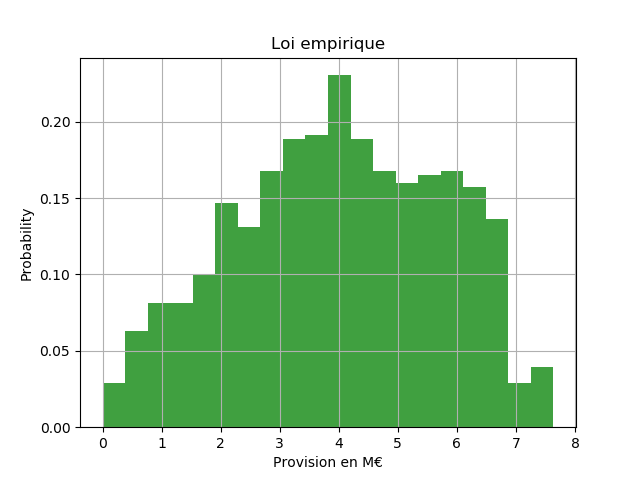
\includegraphics[height=10cm,width=16cm]{Population_homogene/loi_empirique.png}
%\caption{Courbe Euribor juillet 2019}
\end{figure}
Le tableau \ref{per_provision} contient quelques statistiques importantes de la loi empirique de la provision. La loi est assez symétrique, utiliser la moyenne o la médiane comme provision donne presque le même résultat. 
\begin{table}[h!]
	\caption{Loi de la provision.}
	\bigskip	
	\label{per_provision_h}
	\centering
	\csvautotabular{Population_homogene/percentile_provision.csv}
\end{table}

Pour la base de donnes construite dans le chapitre \ref{chap1}, avec estimation de taux de clôtures et des versements par régression non paramétrique, le montant de la provision doit être
$$ provision = 4.00M\mbox{\euro}.$$

La somme des encours de toutes les PEL ouverts en aout 2019 est de 1723M\euro, un peu plus petit que celui de la section précédente, toutefois, la provision est plus importante, 4M\euro. Il s'agit d'une augmentation de 10\% de la provision. 

La prise en compte de variables spécifiques à chaque plan d'épargne peut avoir un impact significatif sur le calcul de la provision.

\section{Provision avec inclusion des résidus}

Dans le chapitre \ref{chap1}, on a testé la performance de la régression non paramétrique et nous avons obtenu, pour le taux de clôture, un coefficient de détermination $R^2$ de $60$\%. Il y a des variables que déterminent les taux de clôture que ne sont pas pris en compte dans le modèle. Le problème n'est pas présente pour le taux de versement car son $R^2$ est de $98$\%. 

Nous avons le résultat suivant qui nous donne l'effet sur la provision avec l'inclusion d'une nouvelle variable explicative.


\begin{prop}
Sous l'hypothèse d'indépendance des résidus dans la régression non paramétrique, l'inclusion d'une nouvelle variable explicative augmente la valeur de la provision.
\end{prop}

\begin{proof}
Dénote par $\Tc(a)$ la variable aléatoire que nous donne le taux de clôture. Soit $\omega$ la variable aléatoire qui contient toute l'information sur le taux de marché (c'est a dire, le $\omega$ dans l'espace de probabilité du modèle G2++. Soit $\psi$ une autre variable aléatoire qui contient l'information sur le taux de marché et des autres variables explicatives. On dénote $\omega \ll\psi$. Lorsque on estime le taux de clôture avec la régression non paramétrique, on est en train de prendre une moyenne, une espérance conditionnelle sachant les variables explicatives :
$$\Tc(a,\omega) = E[\Tc(a)|\omega]\mbox{ et } \Tc(a,\psi) = E[\Tc(a)|\psi]$$
Pour un pel d'age $a$, $n$ mois après:
\begin{eqnarray}
&&\left[1-E(\Tc(a+n)|\omega)+E(\Tv(a+n)|\omega)\right]\nonumber\\
&\times&\left[1-E(\Tc(a+n+1)|\omega)+E(\Tv(a+n+1)|\omega)\right]\nonumber\\
&=&E\left[\left(1-\Tc(a+n)+\Tv(a+n)\right)\right.)\nonumber\\
&\times&\left.\left(1-\Tc(a+n+1)+\Tv(a+n+1)\right)|\omega\right]\nonumber
\end{eqnarray}
De la égalité ci-dessus et la formule (\ref{En}) on obtient que l'encours au mois $n$ est aussi une espérance conditionnelle :
$$\E_n(\omega) = E(\E_n|\omega).$$
Comme l'encours certain ou minimum est déterministe, de la formule (\ref{perte}), on obtient que la perte actualisé est une espérance conditionnelle:
$$ perte(\omega) = E(perte| \omega)= E(E(perte|\psi)|\omega),$$
où on a utilisé le fait $\omega\ll \psi$.
Dans la formule ci-dessus, {\it perte} est une variable aléatoire qui prends en compte toutes les variables explicatives pour le taux de clôture et le taux de versement.
Finalement:
\begin{eqnarray}
E[provision(\omega)]&=&E[max(0,perte(\omega))]\nonumber\\
&=& E[max(0,E[perte|\omega])] \nonumber\\
&=& E[max(0,E[E[perte|\psi]|\omega])] \nonumber\\
&\leq& E[E[max(0,E[perte|\psi])|\omega]]\nonumber\\
&=& E[max(0,E[perte|\psi])|\omega] \nonumber\\
&=&E[provision(\psi)|\omega].\nonumber
\end{eqnarray}
Avec les espérances des deux côtés de l'équation ci-dessus on obtient que la provision calculé avec les variables explicatives de $\omega$ est inférieur a la provision avec les variables explicatives $\psi$.

Il y a un deuxième effet lorsque des variables explicatives sont incluses. Dans la procédure précédente, nous avons supposé que le montant minimum est déterministe, c'est vrai, mais en général, il est pris en fonction de la loi des variables explicatives à travers la formule:
$$\E_n^c = \min_\omega(\E_n(\omega))  $$
 ou en prenant un quantile tel que 97,5\%. 

Avec l'inclusion d'une nouvelle variable explicative, le montant minimum diminue, ce qui augmente encore la provision.
\end{proof}

Nous venons de voir, dans la démonstration du résultat précédent, que l'inclusion de nouvelles variables explicatives dans l'estimation du taux de clôture augmente la valeur grâce à deux effets, le premier est donné grâce à une augmentation sans modifier le montant minimum et le second est donné grâce à la diminution du montant minimum.

Nous verrons l'effet de ajouter toutes les variables explicatives dans le calcul de la provision. Pour ce faire, nous supposons que les résidus de la régression non paramétrique pour le taux de clôture sont indépendants. Cette hypothèse est vraie si l'on tient compte de la façon dont la base "stock\_pel" a été construite. 

Les variables explicatives manquantes peuvent être obtenues en simulant des variables indépendantes de la loi empirique des résidus étudiée au chapitre 2. Mathématiquement, les taux de clôtures seront 
$$\Tc = \Tc(age,ecart\_taux)+ \E$$
avec $\E$ une variable aléatoire $\E$ de loi donné par les résidus du "test data" de la régression non paramétrique. La figure \ref{encours_min_sr_vs_r} montre l'effet dans l'encours certain, de l'inclusion des erreurs pour un pel âgée de 20 ans.



\begin{figure}[!h]
\label{encours_min_sr_vs_r}
\centering
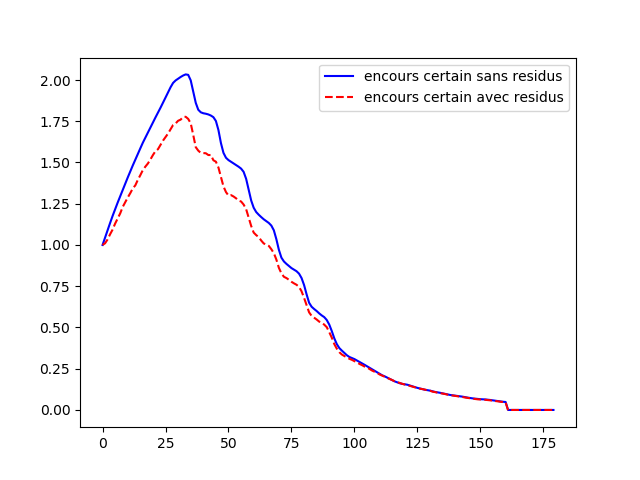
\includegraphics[height=10cm,width=16cm]{encours_min_sr_vs_r.png}
%\caption{Courbe Euribor juillet 2019}
\end{figure}

La loi empirique avec les nouvelles variables explicatives est représenté dans le histogramme suivante :


\begin{figure}[!h]
\label{loi_empirique_e}
\centering
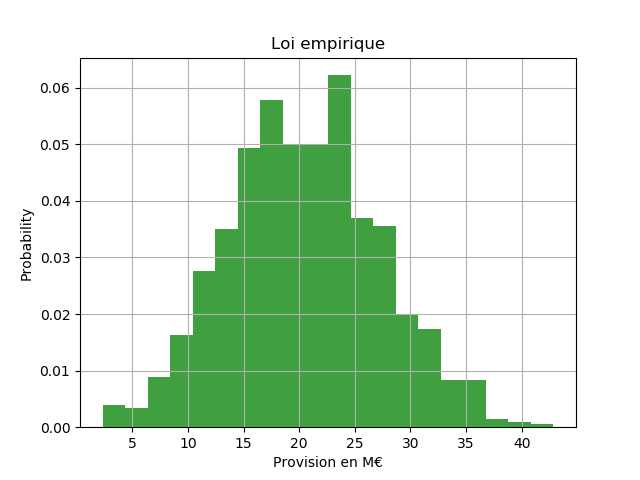
\includegraphics[height=10cm,width=16cm]{loi_empirique_e.png}
%\caption{Courbe Euribor juillet 2019}
\end{figure}

Les statistiques de cette nouvelle loi empirique de la provision sont présentées dans le tableau suivant.

\begin{table}[h!]
	\caption{Loi de la provision.}
	\bigskip	
	\label{per_provision_e}
	\centering
	\csvautotabular{Simulation_encours/percentile_provision_e.csv}
\end{table}

Il convient de noter la grande différence entre cette nouvelle provision et la précédente, calculée sans tenir compte des résidus de la régression non paramétrique: 20.4M\euro{} contre 3.62M\euro. Cela montre que l'inclusion de nouvelles variables explicatives peut avoir un effet significatif sur le calcul de la provision.

\section{Preuve de la proposition \ref{CONV_LIMIT}}

Si on regarde le processus discret a pas mensuel $(X_n,Y_n):=(x_{n/12}, y_{n/12})$, il suffit de démontrer les convergences suivantes: 
\begin{eqnarray}
\lim_{N\rightarrow \infty}\frac{1}{N}\sum_{n=1}^N (X_{n+1}-X_n)^2&=&\sigma ^2 B(a,1/12)\label{x_pearson}\\
\lim_{N\rightarrow \infty}\frac{1}{N}\sum_{n=1}^N (Y_{n+1}-Y_n)^2&=&\eta ^2 B(b,1/12)\label{y_pearson}\\
\lim_{N\rightarrow \infty}\frac{1}{N}\sum_{n=1}^N (X_{n+1}-X_n)(Y_{n+1}-Y_n)&=&\frac{\rho \sigma\eta}{a+b}[aB(a,1/12)+bB(b,1/12)]\nonumber\\
\label{xy_pearson}
\end{eqnarray}
avec la définition de $B$ donné par (\ref{B(z,t)}) : 




Le processus discret a pas mensuel $(X_n,Y_n)$ est une chaine gaussienne où la fonction de covariance converge exponentiellement vers zero. La chaine est "mixing" et donc, ergodique (voir Walters \cite{W}). Grâce au theorem Ergodique nous avons la convergence suivante:
$$\lim_{N\rightarrow \infty} \frac{1}{N}\sum_{n=1}^N (X_{n+1}-X_n)^2 = \lim_{N\rightarrow \infty} \frac{1}{N}\sum_{n=1}^N E(X_{n+1}-X_n)^2 = \lim_{n\rightarrow \infty} E(X_{n+1}-X_n)^2.$$

De l'équation (\ref{x_t}), on obtient $ X_{n+1} = X_n e^{-a/12 } +\sigma \mathcal{N}$, où  

$$ \mathcal{N} = \int_{n/12}^{(n+1)/12}e^{-a((n+1)/12 -u)}d W_u^1$$ est une variable normale centrée, indépendante de $X_n$ et  de variance 
$$ \int_{n/12}^{(n+1)/12}e^{-2a((n+1)/12 -u)}du = \int_0^{1/12} e^{-2au}du = \frac{1-e^{-a/6}}{2a}.$$
De la formule (\ref{x_t}) à nouveau,
$$E[x_n^2]=\sigma^2\int_0 ^ {n/12} e^{-2a(n/12- u)}du= \sigma^2\int_0 ^ {n/12} e^{-2au}du\rightarrow \sigma^2\int_0 ^ {+\infty} e^{-2au}du=\frac{\sigma^2}{2a}.$$
 
Finalement, on trouve la valeur de convergence,
\begin{eqnarray}
E(X_{n+1}-X_n)^2&=&E[X_n^2(e^{-a/12}-1)^2 +\sigma^2 \mathcal{N}^2]\nonumber\\
&\rightarrow & \frac{\sigma^2}{2a}[(e^{-a/12}-1)^2+(1-e^{-a/6})]\nonumber\\
&=&\frac{\sigma^2}{a}(1-e^{-a/12}).\nonumber\\
&=&\sigma ^2 B(a,1/12)\nonumber.
\end{eqnarray}

On a montré (\ref{x_pearson}). Les convergences (\ref{y_pearson}) et (\ref{xy_pearson}) se montrent avec des arguments identiques. 


\section{Conclusions}


Nous avons choisi un modèle de taux d'intérêt à deux facteurs afin de trouver des paramètres qui reproduisent, via la proposition \ref{CONV_LIMIT}, la matrice de variance-covariance empirique obtenue à partir de données historiques de taux d'intérêt de différentes maturités. En particulier, nous avons tenté de reproduire la matrice de variance-covariance associée au taux Euribor 1 an et au taux OAT 5 ans. Comme la matrice est symétrique, il s'agit de trouver 3 valeurs à l'aide de 5 paramètres.

Bien qu'il y ait plus de paramètres que d'équations, nous avons pu reproduire seulement 2 des 3 valeurs avec une précision correcte. Le problème est dû aux restrictions que les paramètres doivent satisfaire. Nous avons préféré négliger la variance de la série donnée par le taux de l'OAT 5 ans. Il est pour nous, plus important de pouvoir reproduire la covariance entre les taux des 2 maturités différentes, sans négliger la variance des taux à court terme. Ce dernier est utilisé dans la modélisation comportementale et dans le calcul de taux d'actualisation.

Nous avons simulé 1000 trajectoires du processus G++, afin d'obtenir les trajectoires probables de taux Euribor à 3 mois et le taux OAT à 10 ans utilisé comme taux de référence pour estimer la perte future de l'établissement financier qui propose le PEL. Nous avons obtenu une estimation de la loi de probabilité associée à la provision qui est assez symétrique. L'utilisation de l'espérance mathématique ou de la médiane comme valeur comptable de la provision laisse des résultats similaires.

Nous avons continué avec l'étude du chapitre \ref{chap1} qui détermine les conséquences de la non prise en compte des variables spécifiques à chaque PEL. Nous estimons que cela produit une provision inférieure de 10 % à celle qui devrait être obtenue en incluant ces variables dans le modèle comportemental.

Nous avons établi et démontré un résultat théorique qui indique que, dans certaines conditions, ignorer les variables explicatives dans la modélisation comportementale produit des valeurs d'estimation de provision inférieures aux valeurs correctes. Ceci est dû à deux effets. Le premier est lié à une augmentation des encours probables et le second est produit par une diminution de l'encours minimum.

Enfin, nous avons essayé de quantifier la perte de valeur de la provision si on ne prend pas en compte certaines variables explicatives. En combinant l'analyse des résidus de régression non paramétrique que nous avons effectuée au chapitre 1\ref{chap1} avec le calcul de la provision, nous concluons que la perte peut être assez importante.


\begin{thebibliography}{99}

\addcontentsline{toc}{chapter}{Bibliographie}

\bibitem{BetAl} Baud N., Demey, P., Jacomy D., Riboulet G., et Roncalli T., 2000. Plan Epargne Logement. Evaluation des Options Cachées d'un PEL. GRO Crédit Lyonnais. 

\bibitem{BT} Bourbonnais, R.,  Terraza M., 2016. Analyse des séries temporelles. 4e éd, Dunod. 

\bibitem{BM} Brigo, D., Mercurio, F., 2006. Interest Rate Models, Theory and Practice. 2nd ed. Springer Finance

\bibitem{CNC1} Conseil National de la Comptabilité, 2006. Avis relatif à la comptabilisation des comptes
et plans d'épargne-logement. Avis N 2006-02 du 31 mars 2006.

\bibitem{CNC2} Conseil National de la Comptabilité, 2006. Avis relatif à la comptabilisation des comptes
et plans d'épargne-logement. Note de présentation - Avis N 2006-02 du 31 mars 2006.

\bibitem{H} Hardle, W., 1990, Applied Nonparametric Regression. Cambridge University Press

\bibitem{HFT} Hastie, T., Friedman J., Tibshirani R.,  2009. Elements of statistical learning: data mining, inference and prediction. Springer-Verlag New York Inc 5e.

\bibitem{S} Schatzman M., 2004. Analyse numérique : Une approche mathématique. Paris Dunod, coll. « Sciences Sup ».

\bibitem{W} Walters, P., 1982. An Introduction to Ergodic Theory. Springer-Verlag New York 
	 
	 %\bibitem{R} Rost, H., 1981. Non-equilibrium behavior of a many particle process: Density profile and local equilibria. Z. Wahrsch. Verw. Gebiete 58, 41-53.

	 
\end{thebibliography}


\appendix



\chapter{Plan d'Épargne Logement}
\label{app_pel}


\section{Plans d’épargne logement.}

Nous présentons les principales caractéristiques des plans d'épargne logement qu'on peut trouver sur le site officiel de l'administration française Service-Public.fr.:

 https://www.service-public.fr/particuliers/vosdroits/F16140

Le plan d'épargne logement (PEL) est une épargne bloquée qui vous permet d'obtenir des intérêts et, sous conditions, une prime d'État et un prêt immobilier après une phase d'épargne d'une durée minimale de 3 ans.
Le montant du crédit accordé dépend des intérêts obtenus : on parle des droits à prêts. Ils correspondent au total des intérêts acquis (hors éventuelle prime d'État), à la date du dernier anniversaire du plan. Ils apparaissent en général sur le relevé de compte. Pour les PEL souscrits avant août 2003, la prime était en effet intégrée dans la rémunération de la phase d'épargne du PEL. Pour les PEL ouverts après cette date, les droits à prêts correspondent à l'ensemble des intérêts bruts perçus.
Avant 2018 les intérêts du PEL étaient exonérés d'impôt sur le revenu, mais soumis aux prélèvements sociaux. Depuis 2018 les intérêts des nouveaux PEL sont entièrement fiscalisés et ne vous permettent plus de bénéficier de la prime d'État.

Le montant du prêt épargne logement est calculé de la manière suivante : Les droits à prêts sont multipliés par un coefficient de 2,5 pour une utilisation classique du crédit. Cela donne un total d'intérêts de remboursement. Ensuite, pour chaque durée entre 2 et 15 ans, on recherche le montant du crédit qui correspond à ce total d'intérêts. Le taux utilisé pour ce calcul est celui de la phase épargne (hors éventuelle prime). Le montant trouvé est plafonné à 92.000 €.

Conditions d'ouverture :  Toute personne, majeure ou mineure, peut être titulaire d'un PEL. Vous ne pouvez être titulaire que d'un seul PEL. Si vous avez un compte épargne logement, vous pouvez souscrire un PEL à condition de le détenir dans le même établissement bancaire. Pour ouvrir un PEL, vous devez signer un contrat écrit avec l'établissement bancaire et verser le montant minimum requis.

Versements :  Le Versement initial est de 225 € minimum. Au cours d'une année, la somme de vos versements doit atteindre le montant minimum de 540 €. Vous pouvez effectuer des versements périodiques dont le montant est fixé par le contrat. En général, ils sont fixés de la manière suivante :

45 € par mois

Ou 135 € par trimestre

Ou 270 € par semestre

Vous pouvez aussi faire des versements exceptionnels.

Plafond : Le plafond du PEL est de 61 200 €.

Durée : La durée minimale du PEL est de 4 ans. Tout retrait avant 4 ans empêche de bénéficier pleinement des avantages du PEL. La durée maximale est de 10 ans. Passé 10 ans, vous ne pouvez plus effectuer de versements, mais votre PEL continue de produire des intérêts pendant 5 ans. S'il a été ouvert à partir du 1er mars 2011, votre PEL est automatiquement transformé en un livret d'épargne classique à la 15e année. La banque fixe le taux de rémunération.

    Renouvellement : Le PEL ouvert à partir de mars 2016 et d'une durée de moins de 10 ans est prolongé automatiquement tous les ans, sauf décision contraire de votre part. L'établissement bancaire vous en informe chaque année, un mois avant la date anniversaire du plan. Cette disposition s'applique à partir de juillet 2016 pour les PEL ouverts avant mars 2016.
    Taux d'épargne et taux du Prêt: Le prêt effectivement accordé aura le taux de la phase épargne (hors éventuelle prime) auquel sont ajoutés « des frais de gestion et des frais financiers » d'un maximum de 1,20\% (ou 1,70\% pour les PEL ouverts jusqu'au 31 janvier 2015). Voir le tableau récapitulatif suivant les générations de PEL ci-dessous.


\begin{table}[h!]
	\caption{\bf Taux PEL}
	\bigskip	
	\label{taux_pel}
	\centering
	\csvautotabular{taux_pel.csv}
\end{table}
\footnotetext[1]{Le taux d'épargne PEL ne comprend plus de prime d'Etat depuis le 1er août 2003.}
\footnotetext[2]{Depuis janvier 2018 le PEL ne permettent plus d'obtenir une prime d'Etat.}


Les intérêts sont capitalisables, c'est-à-dire qu'au 31 décembre de chaque année, ils viennent s'ajouter au capital déjà épargné et deviennent producteurs d'intérêts supplémentaires.
Le taux du prêt indiqué correspond à un taux actuariel annuel, ce qui correspond à la réglementation de l'épargne logement. Les banques doivent utiliser un taux annuel proportionnel (au moins au niveau du taux effectif global) lorsqu'il s'agit de prêt immobilier. Ce taux sera légèrement inférieur. Le formulaire de calcul indique les deux types de taux.
Lorsque des droits à prêts, issus de différents PEL, sont utilisés pour une même opération (par cession des droits à prêts ou donation d'un plan), les droits sont regroupés par génération de taux et calculés indépendamment. Le montant total des prêts accordés (ou d'un seul prêt épargne-logement fusionné) reste limité au plafond de 92.000 €.


Fiscalité : Les intérêts d'un PEL de moins de 12 ans sont exonérés d'impôt sur le revenu mais soumis aux prélèvements sociaux. Les intérêts d'un PEL ouvert depuis plus de 12 ans sont soumis, lors de leur versement, à un prélèvement forfaitaire de 12,8\%. Ces intérêts seront ensuite portés sur votre déclaration de revenus pour être imposés.
Les intérêts du PEL ouvert à partir de 2018 sont soumis, lors de leur paiement, à un prélèvement forfaitaire unique de 30 \%. Ce prélèvement correspond à l'impôt sur le revenu, à hauteur de 12,80 \%, et aux prélèvements sociaux, à hauteur de 17,20 \%.

Obtention du prêt : Sous certaines conditions, vous pouvez utiliser votre PEL pour obtenir un prêt à taux privilégié (voir ci-dessous). Un membre de votre famille peut vous céder ses droits à prêt et vous pouvez les cumuler avec les vôtres pour obtenir un montant d'emprunt plus important. Parallèlement, vous pouvez céder vos droits à prêt à un membre de votre famille, mais à condition qu'il soit titulaire d'un PEL ouvert depuis au moins 3 ans.

Clôture : Tout retrait effectué sur un PEL entraîne la clôture du plan. Pour le retrait intervenu avant 2 ans, les intérêts seront recalculés au taux du CEL en vigueur à la date de clôture et vous perdrez les droits à prêts et à prime. Pour le retrait intervenu entre 2 et 3 ans, vous garderez le bénéfice du taux de rémunération du PEL, mais vous perdrez vos droits à prêts et à prime. Pour le retrait intervenu entre 3 et 4 ans, vous garderez le bénéfice du taux de rémunération du PEL, mais vos droits à prêts et à prime seront diminués. Le retrait effectué après les 4 ans du PEL n'entraîne pas de pénalités. 
Décès du titulaire :  Si le PEL n'est pas parvenu à terme (10 ans) à la date du décès de son titulaire, l'héritier peut reprendre le plan à la condition qu'il tienne l'ensemble des engagements du défunt (durée, montant des versements, etc.). L'héritier disposant déjà d'un PEL ouvert à son nom peut le conserver. Le PEL parvenu à terme au décès du titulaire est clôturé. Si aucun héritier ne reprend le PEL, celui-ci est clôturé.

Compte inactif : Un compte d'épargne est considéré comme inactif si aucune opération n'a été effectuée pendant 5 années consécutives. Chaque année, l'établissement gérant ce compte doit en informer le titulaire.

Si, au bout de 20 ans, le titulaire ou un de ses proches ne s'est pas manifesté, les fonds de ce compte sont obligatoirement transférés à la Caisse des dépôts et consignations (CDC). Elle les conserve pendant 20 ans et si le titulaire ou un de ses ayants-droits ne les a pas réclamés, les fonds sont définitivement conservés par l'État.


\section{Constitution de la Provision}
Le Conseil National de la Comptabilité (Note de présentation-avis No 2006-02 du 31 mars 2006) prévoit que “les engagements aux conséquences défavorables pour les établissements de crédit habilités à recevoir des dépôts d'épargne-logement et à consentir des prêts d'épargne logement doivent être provisionnés à chaque arrêté, ces engagements étant relatifs, d'une part, à l'obligation de rémunérer l'épargne dans le futur à un taux fixé à l'ouverture du contrat pour une durée indéterminée, et, d'autre part, à l'octroi d'un crédit aux souscripteurs des comptes et plans d'épargne-logement à un taux déterminé fixé à l'ouverture du contrat.” (Note de présentation-avis No 2006-02 du 31 mars 2006).
Les provisions doivent être calculées par génération de plans d'épargne logement : Une génération de contrats se définit comme un ensemble de contrats partageant les mêmes caractéristiques réglementaires et, notamment, les mêmes conditions de taux pour les phases "épargne" et "crédit". 
Il n'y a pas de compensation possible entre les engagements relatifs à des générations différentes.
Modalités de constitution de la provision.
Les encours futurs d'épargne et de crédit dépendent du niveau futur des taux et des comportements des épargnants dans les différents contextes possibles de taux. Les paramètres d'estimation des comportements futurs d'épargne et de crédit doivent résulter d'observations historiques de longue période.
La courbe des taux d'intérêt observables sur le marché en date d'évaluation ou celle utilisée par les établissements pour leurs besoins de planification et de gestion constituent la donnée de base pour évaluer les taux futurs. A partir de celle-ci, des modèles de taux peuvent être utilisés pour déterminer différents chemins de taux futurs et quantifier l'encour en risque.
L'encour en risque :  Par rapport aux produits d'épargne classiques, la spécificité des plans d'épargne-logement réside dans l'incertitude sur le niveau de l'encours futur et son évolution dans le temps sachant que la rémunération de l'encours d'épargne des plans d'épargne-logement est fixée dès l'origine du contrat.
Cette incertitude est notamment due au niveau des taux du marché, dont dépend le comportement des clients. Elle concerne non seulement le rythme des versements que les clients peuvent effectuer jusqu'à la dixième année, mais également le niveau des retraits de la totalité de l'épargne liés ou non à l'utilisation des droits à prêts.
En raison de ces incertitudes, le niveau d'épargne minimum attendue et le niveau d'épargne probable sont déterminés statistiquement en tenant compte des observations historiques des comportements effectifs des clients. L'encours futur minimum évalué statistiquement sous un intervalle de confiance très élevé ne diffère pas, au plan comptable, d'un portefeuille de dépôts à terme, n'ayant aucun caractère optionnel. Il doit en conséquence demeurer comptabilisé à la valeur nominale de ses constituants. La fraction de l'encours incertain qui génère un risque est dite "encours d'épargne en risque".






\chapter{Taux d'intérêts}

\begin{table}[h!]
	\caption{\bf Taux Euribor 3 mois}
	\bigskip	
	\label{eur3m}
	\centering
	\csvautotabular{euribor3m.csv}
\end{table}

\begin{table}[h!]
	\caption{\bf Taux Euribor 1 an}
	\bigskip	
	\label{eur1a}
	\centering
	\csvautotabular{euribor1a.csv}
\end{table}



\chapter{Code python}


\section{client.py}
\label{client.py}
Le module client.py contient le code python pour créer un plan épargne logement avec date de ouverture entre janvier 1999 et aout 2019. Les donnés historiques comme le taux euribor et le taux des plan d'épargne logement sont obtenues a partir du module get\_data.py.  L'objet principal du code est la classe Client avec les trois paramètres de base : mois de origine, montant souhaite et durée souhaite.

On peut simuler un PEL avec le code

\begin{verbatim}
 >>> pel = Client(mois_origine = 10, montant_souhaite=30000, 
 				  duree_souhaite=60)
\end{verbatim}

Pour simuler l'encours du PEL precedente, on utilise le code:

\begin{verbatim}
>>> pel.simulation_encours()
\end{verbatim}

\medskip

{\bf \underline{Fichier code.py}}:
\begin{small}
\begin{verbatim}

import get_data as gd
import numpy as np
import time

class Client:
    def __init__(self, mois_origine, montant_souhaite,
                 duree_souhaite):
        '''
        mois_origine c'est le mois de ouverture du pel... le mois i
        correspond a i mois après janvier 1999. Le mois 0 est janvier 1999.

        montant_souhaite est le montant a épargner prévue :
        c'est un valeur entre 10000 et 61200 (le plafond du PEL)

        duree_souhaite = la duree prevue par le client de la phase epargne
        logement.
        '''

        self.tx_epargne = gd.taux_epargne_PEL(num_mois=mois_origine)
        self.tx_pret = gd.taux_pret_PEL(num_mois=mois_origine)
        self.mois_origine = mois_origine

        # le rendement mensuel de la phase epargne est donc
        r = (1 + self.tx_epargne) ** (1 / 12) - 1

        self.tx_epargne_mensuel = r

        # la mensualite pour arrive au montant suhaite dans la duree souhaite
        self.montant_souhaite = montant_souhaite
        self.mensualite = r * montant_souhaite / ((1+r) ** duree_souhaite - 1)

    def simulation_encours(self, RS):
        '''
        funcion pour simuler les encours, versement et clotures
        du pel, en funcion du conditions du marche du contrat
        pel. RS est un numpy random state pour le seed.
        '''

        if RS is None:
            RS = np.random.RandomState()

        r = self.tx_epargne_mensuel

        encours = [self.mensualite]  # c'est l'encours a la date d'ouverture

        versements = [self.mensualite]  # le premier mois il n'a pas de
        # versement exceptionnel.

        clotures = [0]  # c'est l'ouverture du PEL, donc il n y a pas de
        # cloture

        dernier_mois = min(self.mois_origine + 179, 247)  # c'est le dernier
        # mois a simuler :  soit le pel arrive a l'age maximal de 180 mois,
        # soit le pel arrive au mois actuel; le mois 248 = aout 2019.

        for mois in range(self.mois_origine + 1, dernier_mois + 1):
            if encours[-1] == 0:
                # si le dernier montant des encours est 0, le PEL est fermee,
                # il n y a pas donc des versements ni clotures pour les mois
                # suivantes.
                encours += [0]
                versements += [0]
                clotures += [0]
            else:
                # On calcule si le clien veut cloturer le pel.
                # Le taux de cloture annuel est definie comme p + ref, avec
                # p une variable qui depend de l'age du pel et ref une variable
                # qui depend des taux du pel et des conditions de marche.
                # On prend ref = 5*(taux marche -taux pel). Plus grande ref,
                # plus grand le desir de cloturer le PEL.
                # Par example: Si taux_marche - taux_pel est de 10%
                # (un grand ecart) le taux de cloture annuel va aumenter
                # 50 pbs.
                # Le taux de marche a comparer avec le taux est :
                # 0.02 + 0.25 * euribor_1a (la regression linaire fait dans
                # get_data.py)

                taux_marche = 0.02 + 0.25 * gd.euribor_1a[mois]
                ref = 5 * (taux_marche - self.tx_epargne)

                age_pel = mois - self.mois_origine
                if age_pel < 48:
                    cloturer_pel = veut_cloturer(age_pel=age_pel,
                                                 taux_pel=self.tx_epargne,
                                                 ref=ref,
                                                 RS=RS
                                                 )
                else:
                    cloturer_pel = veut_cloturer(
                        age_pel=age_pel,
                        taux_pel=self.tx_epargne,
                        ref=ref,
                        RS=RS,
                        montant_souhaite=self.montant_souhaite,
                        encours_2=encours[-2],
                        encours_1=encours[-1]
                        )

                if cloturer_pel:
                    clotures += [min(encours[-1]*(1+r), 61200)]
                    versements += [0]
                    encours += [0]
                else:
                    if round(encours[-1] * (1+r), 4) >= 61200:
                        # l'encours du pel est plafonee a 61200.
                        encours += [61200]
                        versements += [0]
                        clotures += [0]
                    else:
                        # le montant a verser va incrementer si le taux
                        # marche es base par rapport au taux du pel, c'est
                        # a dire si -ref est eleve.
                        if age_pel < 120:
                            montant_verser = self.mensualite\
                                        * max(1, 1-ref+0.25 * RS.normal())
                        else:
                            montant_verser = 0

                        versements += [min(61200 - encours[-1] * (1+r),
                                           montant_verser)]
                        clotures += [0]
                        encours += [encours[-1] * (1 + r) + versements[-1]]

        self.encours = np.array(encours)
        self.versements = np.array(versements)
        self.clotures = np.array(clotures)


def veut_cloturer(age_pel,
                  taux_pel,
                  ref,
                  RS=None,
                  montant_souhaite=None,
                  encours_2=None,
                  encours_1=None,
                  taux_marche=None):

    '''
    resultat de la funcion = True si le client cloture le pel,
    = False si ne le souhaite pas. La variable encours_2 est
    l'encours du pel 2 mois avant et encours_1 celui du mois
    precedent. Les 2 variables vont determiner si le
    client vient de attend son objectif = montant souhaite.
    
    RS= numpy random state pour le seed.
    La variable ref (reference) est la variable de adjustment.
    Il change le taux de cloture en function du marche et du
    taux pel. Le taux cloture annuel est  p + ref.
    '''

    if age_pel < 24:
        p = 1 - (max(0, 0.975 - ref)) ** (1 / 12)  # le taux cloture
        # est de 2.5% annuel le deux premiers annes de ouverture du pel
    elif age_pel < 48:
        p = 1 - (max(0, 0.95 - ref)) ** (1 / 12)  # 5% annuel avant le 4 anne.
    else:
        if round(encours_1, 4) < montant_souhaite:
            # le client n'a pas encore arriver a epargner le
            # montant souhaite, le taux cloture est de 10%
            # annuel.
            p = 1 - (max(0, 0.9 - ref)) ** (1 / 12)
        elif round(encours_2, 4) < montant_souhaite:
            # le client vient d'arriver a epargner son montant
            # souhaite. Sont taux cloture est de 60 %
            p = min(1, 0.6 + ref)
        else:
            # si le client ne cloture pas le pel quand arrive
            # a epargner le montant souhaite, alors il va le
            # cloture aux taux de 30% annuel
            p = 1 - (max(0, 0.7 - ref)) ** (1/12)

    if RS is None:
        RS = np.random.RandomState()

    return RS.uniform() < p

\end{verbatim}
\end{small}


\section{get\_data.py}
\label{get_data.py}

C'est le module pour obtenir les donnes historiques a utiliser : Le taux euribor a 1 an, 3 mois et les taux des Plan d'Epargne Logement.

\medskip

{\bf \underline{File get\_data.py}}:
\begin{small}
\begin{verbatim}
import pandas as pd
import numpy as np
import matplotlib.pyplot as plt


def obtenir_taux(string):
    '''
    string = 'Euribor 3M.txt' ou 'Euribor 1A.txt' pour le taux
    euribor 3 mois ou 1 an respectivement.
    la function return la liste a avec le taux euribor mois par mois
    depuis janvier 1999.
    '''
    euribor = pd.read_csv(string, sep='\t')

    # ====================================================
    # On transforme la matriz euribor_3m a une liste
    vecteur = []
    for annee in map(str, range(1999, 2020)):
        vecteur += list(euribor[annee].values / 100)

    # on elimine les derniers 4 valeurs manquantes
    return vecteur[:-4]

# on obtient le taux euribor 3m et euribor 1 an :
euribor_3m = obtenir_taux('Euribor 3M.txt')
euribor_1a = obtenir_taux('Euribor 1A.txt')

def taux_epargne_PEL(mois=None, anne=None, num_mois=None):
    '''
    donne le taux pel de la phase epargne pour un PEL ouvert a la date
    mois/anne. On ne considere que des PEL ouverts apres 1999.
    La variable num_mois est la date en nombre de mois depuis janvier
    1999. (janvier 1999 est num_mois = 0)

    Par example : Pour obtenir le taux PEL de la phase epargne de un PEL
    ouvert en juin 2000, on peut ecrire taux_epargne_PEL(6, 2000) ou
    taux_epargne_PEL(num_mois=17)

    '''
    if num_mois is None:
        num_mois = (anne-1999) * 12 + mois

    if num_mois < 7:
        return 2.9/100
    elif num_mois < 30:
        return 2.61/100
    elif num_mois < 55:
        return 3.27/100
    elif num_mois < 193:
        return 2.5/100
    elif num_mois < 205:
        return 2/100
    elif num_mois < 211:
        return 1.5/100
    else:
        return 1/100

def taux_pret_PEL(mois=None, anne=None, num_mois=None):
    '''
    Pour detailles des variables voir la function taux_epargne_PEL
    Le taux de  pret du PEL est egale a le taux de phase + 1.7% pour
    les PEL ouvert avant fevrier 2015 ou  + 1.2% pour le PEl ouvert
    avant
    '''
    if num_mois is None:
        num_mois = (anne-1999)*12 + mois

    if num_mois <= 193:
        return taux_epargne_PEL(mois=mois, anne=anne, num_mois=num_mois)\
                              + 1.7 / 100
    else:
        return taux_epargne_PEL(mois=mois, anne=anne, num_mois=num_mois)\
                              + 1.2 / 100

# on obtient une liste avec le taux pel de epargne et pret pour les 248
# mois de janvier 1999 a aout 2019.

taux_pel_epargne = []
taux_pel_pret = []
for k in range(248):
    taux_pel_epargne += [taux_epargne_PEL(num_mois=k+1)]
    taux_pel_pret += [taux_pret_PEL(num_mois=k+1)]


# on regarde graphiquement la relation entre le taux pel (phase epargne)
# et le taux Euribor 1 an.
if __name__ == '__main__':
    t = np.arange(248)
    # plt.plot(t, np.array(euribor_1a), '--', label="euribor",  t,  # 'bs'
    #          np.array(taux_pel_epargne), '.-', label="taux pel")  # 'g^'
    plt.plot(t, np.array(euribor_1a), color="blue",
             linewidth=1.5, linestyle="--", label="euribor")
    plt.plot(t, np.array(taux_pel_epargne), color="red",
             linewidth=1.5, linestyle="-.", label="taux pel")
    plt.legend(loc='upper right')
    plt.show()

    # =========================================================================
    # soit x le taux euribor  1 an et y le taux pel (phase epargne). Pour
    # choisir le taux pel, on considere le taux euribor 1 an comme
    # un proxi du marche. Il y a une relation entre le taux pel et le taux
    # euribor : y = a + bx + e. On calcule les coeficients a et b par moindre
    # carres :

    x = np.array(euribor_1a)
    y = np.array(taux_pel_epargne)
    matriz_var = np.cov(x, y)
    b = matriz_var[0, 1] / matriz_var[0, 0]
    a = y.mean() - b * x.mean()
    print([a, b])
    coef_correlation = b * x.std() / y.std()
    print(coef_correlation)

    # donc a = 0.02 et b = 0.25. Le coefficient de correlation entre le taux
    #  euribor et le taux pel est 0.66.

    # Commentaire: pour le cloture et les versements exceptionels, le gens
    # prend en consideration le taux pel par rappor au conditions du marche.
    # Le proxi du marche a utiliser est, du au regression lineaire decrit
    # precedement :
    # r = 0.02 +0.25*taux_euribor_1a. Si taux_pel-r est eleve le gens realisent
    # des versement exceptionnels et peut de clotures. Au contraire, si
    # taux_pel-r est basse (le conditions du marche sont plus rentables que les
    # taux pel du contrat... qui va rester fixe), le gens vont cloturer le pel
    # et realiser peu des versements exceptionnels.

\end{verbatim}
\end{small}

\section{regression\_non\_paramtrique.py}
\label{non_parametric_regression.py}
\begin{small}
\begin{verbatim}
'''
module que calcule la regression non parametrique o kernel regression
'''

import numpy as np
from sklearn.model_selection import train_test_split


class Kernel:
    def __init__(self, X, Y, h=None, test_size=1/3, RS=None):
        '''
        X est une matriz (numpy 2D array) avec les variables explicatives

        Y est la variable independante.

        h est la fenetre de lissage pour le vecteur des observations.

        f est la function kernel a utiliser : f = gaussienne par default.

        RS le numpy random state pour avoir la seed
        '''
        if test_size == 0:
            self.X_train = X
            self.X_test = None
            self.Y_train = Y
            self.Y_test = None
        else:
            (self.X_train,
             self.X_test,
             self.Y_train,
             self.Y_test) = train_test_split(X,
                                             Y,
                                             test_size=test_size,
                                             random_state=RS)
        self.h = h

    def y_hat(self, x, h=None):
        '''
        donne le valeur estime du y associe a une observation x
        de la regression non parametrique avec function kernel
        f (gaussien par default) et h la fenetre de lissage fenetre.
        x et h sont de largeur le nombre de colonnes des observatios X.
        La regression non parametrique utilise uniquement les
        observations du train data.
        '''

        num_obs, num_var = self.X_test.shape
        if h is None:
            h = self.h

        product = np.ones(num_obs)
        for i in range(num_var):
            Z_i = np.exp(-((self.X_test[:, i] - x[i]) / h[i])**2)
            product = product*Z_i

        return np.inner(self.Y_test, product)/product.sum()

    def Y_hat(self, X, h=None):

        Y_hat = []

        for x in list(X):
            Y_hat += [self.y_hat(x=x, h=h)]

        return np.array(Y_hat)

    def R2(self, X=None, Y=None, h=None):
        '''
        Return le coefficient de determination R2, base sur la
        performance du model sur les observations X, Y (test data
        par default).
        '''
        if X is None or Y is None:
            X = self.X_test
            Y = self.Y_test

        if Y is not None:
            Y_hat = self.Y_hat(X=X, h=h)
            return(R2(Y, Y_hat))
        else:
            return(None)


def R2(Y, Y_hat):
    return 1 - (1 / Y.size) * ((Y - Y_hat) ** 2).sum() / Y.var()
\end{verbatim}
\end{small}

\section{gpp.py} \label{gpp.py}
\begin{small}
\begin{verbatim}


import numpy as np
import pandas as pd
import matplotlib.pyplot as plt
from scipy.interpolate import interp1d


def B(z, t):
    return (1 - np.exp(-z * t)) / z


def V(t, a, b, sigma, eta, rho):
    S1 = ((sigma ** 2) / (a ** 2)) * (t - 2 * B(a, t) + B(2 * a, t))
    S2 = ((eta ** 2) / (b ** 2)) * (t - 2 * B(b, t) + B(2 * b, t))
    S3 = (2 * rho * sigma * eta / (a * b)) * \
         (t - B(a, t) - B(b, t) + B(a + b, t))
    return S1 + S2 + S3


def cov_theorique(T1, T2, a, b, sigma, eta, rho):
    S1 = (sigma ** 2) * B(a, 1 / 12) * B(a, T1) * B(a, T2) / (T1 * T2)
    S2 = (eta ** 2) * B(b, 1 / 12) * B(b, T1) * B(b, T2) / (T1 * T2)
    S3 = rho * eta * sigma / (a + b) *\
        (a * B(a, 1 / 12) + b * B(b, 1 / 12)) *\
        (B(a, T1) * B(b, T2) + B(b, T1) * B(a, T2)) / (T1 * T2)

    return S1 + S2 + S3


def mcov_theorique(T, a, b, sigma, eta, rho):
    '''
    calcul de la matriz de variance covariance theorique.
    T est une liste avec les maturites
    '''
    n = len(T)
    matrice = np.zeros([n, n])
    for i in range(n):
        for j in range(n):
            T1 = T[i]
            T2 = T[j]
            matrice[i, j] = cov_theorique(T1, T2, a, b, sigma, eta, rho)

    return matrice


class G2pp:
    '''
    class qui simule une trajectoire (x_t, y_t) du modele G2++
    '''

    def __init__(self, a, b, sigma, eta, rho):
        self.a = a
        self.b = b
        self.sigma = sigma
        self.eta = eta
        self.rho = rho
        self.X = np.array([])
        self.Y = np.array([])

    def simula(self, x0=0, y0=0, pas=1/12, num_pas=12, RS=None):
        '''
        pas le pas de la simulation, on simule par mois
        par defaut.

        num_pas= nombre de variable a simuler dans la trajectoire.

        RS = numpy random state pour tracker la seed.
        '''
        if RS is None:
            RS = np.random.RandomState()

        Z = [[x0, y0]]
        for t in range(num_pas - 1):
            x = Z[-1][0]
            y = Z[-1][1]

            m_cov = [
                     [self.sigma ** 2 * B(2 * self.a, pas),
                      self.rho * self.sigma * self.eta *
                      B(self.a + self.b, pas)],
                     [self.rho * self.sigma * self.eta *
                      B(self.a + self.b, pas),
                      self.eta ** 2 * B(2 * self.b, pas)]
                ]

            m_cov = np.array(m_cov)

            N = RS.multivariate_normal(mean=np.array([0, 0]), cov=m_cov)

            x1 = x*np.exp(-self.a*pas) + N[0]

            y1 = y*np.exp(-self.b*pas) + N[1]

            Z += [[x1, y1]]

        Z = np.array(Z)
        return Z

    def simula_XY(self, x0=0, y0=0, pas=1/12, num_pas=12, num_sim=1, RS=None):
        X = []
        Y = []
        for i in range(num_sim):
            Z = self.simula(x0, y0, pas, num_pas, RS)
            X += [Z[:, 0]]
            Y += [Z[:, 1]]
        return (np.array(X), np.array(Y))  # X.shape = [num_sim, num_pas]

    def add_XY(self, x0=0, y0=0, pas=1/12, num_pas=12, num_sim=1, RS=None):
        (X, Y) = self.simula_XY(x0, y0, pas, num_pas, num_sim, RS)
        self.X = X
        self.Y = Y
        self.pas = pas

    def taux(self, maturite, courbe, pas=1/12, num_pas=12,
             num_sim=None, RS=None):
        '''
        simule le trajectoires du taux avec courbe initial f^M=courbe
        et a maturite T. Courbe = f est une fonction t --> f^M(0,t)
        '''

        if num_sim is None:
            X = self.X
            Y = self.Y
            pas = self.pas
            num_sim = X.shape[0]
            num_pas = X.shape[1]

        else:
            (X, Y) = self.simula_XY(x0=0, y0=0, pas=pas,
                                    num_pas=num_pas,
                                    num_sim=num_sim, RS=None)

        T = maturite
        f = np.array([(T + n * pas) * courbe(T + n * pas) -
                     n * pas * courbe(n * pas)
                     for n in range(num_pas)])
        para = [self.a, self.b, self.sigma, self.eta, self.rho]
        Vt = -0.5 * V(T, *para) + 0.5 * np.array([V(T + n * pas, *para) -
                                                 V(n * pas, *para)
                                                 for n in range(num_pas)])

        return (f + Vt + B(self.a, T) * X + B(self.b, T) * Y) / T

if __name__ == '__main__':

    # les valeurs del example de la section 4.2.7 de [BM]
    a, b, sigma, eta, rho = 0.77, 0.082, 0.02, 0.01, -0.7

    # on va simuler 7 trajectoires de taux OAT 3 mois avec la
    # courbe inital OAT de juillet 2019.

    mois = np.array([0, 1, 3, 6, 9, 12, 24, 60, 120, 360]) / 12
    OAT = np.array([-0.4102903226,
                    -0.4102903226,
                    -0.409483871,
                    -0.4404516129,
                    -0.4866451613,
                    -0.4727096774,
                    -0.5133225806,
                    -0.4129354839,
                    -0.0512032258,
                    0.6592903226])

    f_OATi = interp1d(mois, OAT / 100, kind='cubic')

    def f_OAT(t):
        return float(f_OATi(min(t, 30)))

    # on fait un graphique de la courbe de taux avec kernel regression
    m = np.array(range(360)) / 12
    taux = list(map(f_OAT, m))
    plt.plot(m, taux, label="courbe OAT juillet 2019")
    plt.legend(loc='upper left')
    plt.show()

    g2pp = G2pp(a=a, b=b, sigma=sigma, eta=eta, rho=rho)

    RS = np.random.RandomState(19032015)
    g2pp.add_XY(num_pas=120, num_sim=10, RS=RS)
    R1 = g2pp.taux(maturite=3 / 12, courbe=f_OAT)
    R2 = g2pp.taux(maturite=1, courbe=f_OAT)

    cv = cov_theorique(3 / 12, 1, a, b, sigma, eta, rho)

    estimateur = []
    for i in range(10):
        estimateur += [((R1[i, 1:]-R1[i, :-1]) *
                       (R2[i, 1:]-R2[i, :-1])).mean() / cv]

    print(estimateur)

    print(cv)

    # ==============================================================
    # Pour le calcul de la provision, on va generer 1000 simulations
    # de 180 mois de observations de taux euribor 3 mois et euribor
    # 10 ans. Le donnes pour le taux 1 semaine, 1, 3, 6 et 12 mois
    # juillet 2019 sont pris du site
    # https://fr.global-rates.com/taux-de-interets/euribor/2019.aspx
    # toutes les taux sont negative on ajoute a taux a 30 ans a 0%
    # ==============================================================

    # courbe inital euribor de juillet 2019.

    mois = np.array([0, 12/52, 1, 3, 6, 12, 24]) / 12
    euribor = np.array([-0.402,
                        -0.402,
                        -0.395,
                        -0.365,
                        -0.347,
                        -0.283,
                        0])

    f_euribori = interp1d(mois, euribor / 100, kind='cubic')

    def f_euribor(t):
        return float(f_euribori(min(t, 2)))

    m = np.array(range(14)) / 12
    taux = list(map(f_euribor, m))
    plt.plot(m, taux, label="courbe euribor juillet 2019")
    plt.legend(loc='upper left')
    plt.show()

    RS = np.random.RandomState(19032015)
    g2pp.add_XY(num_pas=180, num_sim=1000, RS=RS)
    simu_euribor3m = g2pp.taux(maturite=3 / 12, courbe=f_euribor)
    simu_oat10a = g2pp.taux(maturite=10, courbe=f_OAT)

    np.savetxt('simulation_OAT', simu_oat10a)
    np.savetxt('simulation_Euribor', simu_euribor3m)

else:
    simu_euribor3m = np.loadtxt('simulation_Euribor')
    simu_oat10a = np.loadtxt('simulation_OAT')


\end{verbatim}
\end{small}




\section{pel.py}
\begin{small}
\begin{verbatim}
'''
module pour construire la classe Pel, que define une compte d'épargne
logement d'un mois d'origine donné. Les elements de la classe simulent
leur encours par rapport au simulations de Monte Carlo du modèle G2++
obtenu dans le module gpp.py
'''

import numpy as np
from comportemental.get_data import taux_epargne_PEL, euribor_3m
from simulation_taux.gpp import simu_euribor3m, simu_oat10a
from comportemental.nappe import tx_clotures, tx_versements
from comportemental.simulation_erreurs import erreurs_simule
import matplotlib.pyplot as plt

[num_sim, num_mois] = simu_euribor3m.shape


class Pel:
    def __init__(self, age, encours0=1, erreurs=False):
        '''
        class qui contient a generation de PEL, age, c'est
        l'age du PEL ajourhui, et encours le montant du PEL.
        L'age doit etre inferieur a 178 car un pel de 179 mois
        se ferme le mois prochain, donc il faut pas le prendre
        en compte pour la provision.
        '''

        self.age = age
        self.encours0 = encours0
        mois_pel = 247 - age  # mois d'origine de pel, aout 2019
        # est le mois 247. Janvier 1999 le mois 0.
        self.taux_pel = taux_epargne_PEL(num_mois=mois_pel)
        self.encours = self.get_encours(erreurs)

    def taux_clotures(self, erreurs=False):
        tx_cl = []
        for simu in range(num_sim):
            tx_cl_i = []
            for mois in range(num_mois):
                if erreurs:
                    E = erreurs_simule[simu, mois]
                else:
                    E = 0

                tx = tx_clotures(self.age + mois,
                                 simu_euribor3m[simu, mois] -
                                 self.taux_pel) + E

                tx_cl_i += [tx]

            tx_cl += [tx_cl_i]

        return np.array(tx_cl)

    def taux_versements(self):
        tx_vs = []
        for simu in simu_euribor3m:
            tx_vs_i = [tx_versements(self.age + i, simu[i] - self.taux_pel)
                       for i in range(num_mois)]
            tx_vs += [tx_vs_i]
        return np.array(tx_vs)

    def get_encours(self, Erreurs=False):
        encours = self.encours0 * np.ones([num_sim, 1])
        versements = self.taux_versements()
        clotures = self.taux_clotures(Erreurs)

        for mois in range(num_mois - 1):
            encours = np.append(encours,
                                (encours[:, -1] +
                                 encours[:, -1] * (versements[:, mois] -
                                                   clotures[:, mois])
                                 ).reshape(num_sim, 1),
                                axis=1)

        return encours

    def provision(self, q=0):
        '''
        q es le percentile
        '''
        return (DF * (self.encours - np.percentile(self.encours,
                                                   q=0, axis=0)) *
                (1 / 12) * (self.taux_pel - taux_ref)).sum(axis=1)


if __name__ == '__main__':
    # ==============================================================
    # on va faire un graphique de une surface en risque :
    #  encours probable - encours certain
    pel = Pel(20, erreurs=True)
    t = np.arange(180)
    plt.plot(t, np.percentile(pel.encours, q=97.5, axis=0), color="blue",
             linewidth=1.5, linestyle="-", label="encours probable")
    plt.plot(t, np.percentile(pel.encours, q=2.5, axis=0), color="red",
             linewidth=1.5, linestyle="--", label="encours certain")
    plt.legend(loc='upper right')
    plt.show()

# ==============================================================
# taux d'acutalisation : du CNC, euribor 3m moyennes sur 12 mois

if __name__ == '__main__':
    euribor = euribor_3m[-13:-2] * np.ones([num_sim, 11])
    euribor = np.append(euribor, simu_euribor3m, axis=1)
    for i in range(num_mois):
        euribor[:, -i-1] = euribor[:, -i-13:-i-1].mean(axis=1)

    euribor_3m_moy = euribor[:, 11:]

    # Les factor d'actualisation d'un mois au mois i est egale a :

    Pij = (1 / (1 + euribor_3m_moy)) ** (1 / 12)

    # Les factors d'actualisation s'obtient de la formule
    # P0j = P0,1 * P1,2 * P2,3 * ... * Pj-1,j

    DF = np.ones([num_sim, num_mois])
    for i in range(1, num_mois):
        DF[:, i] = DF[:, i-1] * Pij[:, i-1]

    np.savetxt('Discount Factor', DF)

    # on fait un graphique de deux simulations de factor de discount.
    t = np.arange(180)
    plt.plot(t, DF[0], color="blue",
             linewidth=1.5, linestyle="-", label="DF pour siulation 0")
    plt.plot(t, DF[1], color="red",
             linewidth=1.5, linestyle="--", label="DF pour siulation 1")
    plt.legend(loc='upper right')
    plt.show()

else:
    DF = np.loadtxt('Discount Factor')

# ==================================================================
# taux reference : On prend le taux OAT 10 ans plafonée a 0.75% (plafond
# du livret A historique. C'est le gouvernement qui decide le taux)
# Son taux est déterminé par une formule liée aux taux courts et à l’inflation,
#  mais la Banque de France peut proposer au gouvernement de déroger
# exceptionnellement à la règle. Ce taux sert de référence pour déterminer
# les taux de plusieurs autres supports d’épargne réglementée.
# Depuis août 2015, le taux du Livret A est de 0,75%.

taux_ref = np.maximum(simu_oat10a, 0.75 / 100)

if __name__ == '__main__':
    # on fait un graphique de deux simulations de factor de discount.
    t = np.arange(180)
    plt.plot(t, taux_ref[0], color="blue",
             linewidth=1.5, linestyle="-", label="Taux Ref pour siulation 0")
    plt.plot(t, taux_ref[1], color="red",
             linewidth=1.5, linestyle="--", label="Taux Ref pour siulation 1")
    plt.legend(loc='upper right')
    plt.show()

\end{verbatim}
\end{small}







\end{document}

Comentarios a agregar en la conclusion:

el coeficiente de correlation entre l'ecart de taux euribor 3m et taux pel et le taux de versement est de 0.2 et de -0.15 pour le taux de cloture. Son bajos pero hay que tomar en consideracion que estamos en un periodo de tasas de interes bajas, que presentan poca variabilidad, los resultados no permiten excluir las tasas de interes como variables explicativas (también porque es una exigencia del CNC)


Hablar de la dessaisonalisation des variables et de la fiscalisation... on ne le prend pas en compte pour simplifier. 


Voici les parametres: 
 {'a': 0.4022951071294538, 'b': 0.8957603876433327, 'sigma': 0.02637859459387959, 'eta': 0.027301688789222456, 'rho': -0.9862209250670384} 

La matriz de convariance avec les parametres precedentes
       est en termes de porcentages de la matriz observe : 

[[0.80247396 0.82060029 1.38953354]
 [0.82060029 0.98917673 1.49508893]
 [1.38953354 1.49508893 0.33670967]]
[[1.81147308e-06 1.68014361e-06 5.80716629e-07]
 [1.68014361e-06 2.34015725e-06 1.34414909e-06]
 [5.80716629e-07 1.34414909e-06 1.01612900e-06]]
[[2.25736057e-06 2.04745675e-06 4.17921996e-07]
 [2.04745675e-06 2.36576254e-06 8.99042902e-07]
 [4.17921996e-07 8.99042902e-07 3.01781951e-06]]

[Done] exited with code=0 in 555.22 seconds




Voici les parametres: 
 {'a': 0.9950675070110541, 'b': 0.29446719122580156, 'sigma': 0.011848895923549096, 'eta': 0.0094954951375944, 'rho': -0.8485206872738472} 

La matriz de convariance avec les parametres precedentes
       est en termes de porcentages de la matriz observe : 

[[1.14233741 0.93136613 0.87874253]
 [0.93136613 0.69311748 0.60932079]
 [0.87874253 0.60932079 0.12746512]]
[[2.57866743e-06 1.90693187e-06 3.67245833e-07]
 [1.90693187e-06 1.63975136e-06 5.47805529e-07]
 [3.67245833e-07 5.47805529e-07 3.84666714e-07]]
[[2.25736057e-06 2.04745675e-06 4.17921996e-07]
 [2.04745675e-06 2.36576254e-06 8.99042902e-07]
 [4.17921996e-07 8.99042902e-07 3.01781951e-06]]

Voici les parametres: 
 {'a': 0.17400786696273207, 'b': 0.6017037880307475, 'sigma': 0.007322741001897781, 'eta': 0.011437467204373775, 'rho': -0.7647292851848597} 

La matriz de convariance avec les parametres precedentes
       est en termes de porcentages de la matriz observe : 

[[1.0698945  1.22919587]
 [1.22919587 0.2764792 ]]
[[2.53111632e-06 1.10509983e-06]
 [1.10509983e-06 8.34364317e-07]]
[[2.36576254e-06 8.99042902e-07]
 [8.99042902e-07 3.01781951e-06]]

[Done] exited with code=0 in 258.806 seconds



Voici les parametres: 
 {'a': 0.9974929463539162, 'b': 0.007729401185027407, 'sigma': 0.01089724774414369, 'eta': 0.004423827345136688, 'rho': -0.5988234059910441} 

La matriz de convariance avec les parametres precedentes
       est en termes de porcentages de la matriz observe : 

[[1.06051337 0.99912332]
 [0.99912332 0.34566647]]
[[2.50892281e-06 8.98254726e-07]
 [8.98254726e-07 1.04315903e-06]]
[[2.36576254e-06 8.99042902e-07]
 [8.99042902e-07 3.01781951e-06]]

[Done] exited with code=0 in 263.575 seconds

